%!TEX root = ../doc.tex
\documentclass[../doc.tex]{subfiles}

\begin{document}
\chapter{Mixed Finite Element VEF Discretizations} \label{chap:rtvef}
Mixed finite element methods are a class of discretization techniques for solving the mixed variational form of a partial differential equation. This variational form is characterized by the inclusion of multiple (typically two) physically disparate quantities resulting in a saddle point problem \cite{mfem_boffi}. By contrast, primal formulations operate on a single quantity and produce minimization problems. Mixed methods were invented to 1) allow incorporation of a constraint (e.g.~divergence free velocity in fluid flow), 2) provide direct access to an intermediate variable (e.g.~the stress in elasticity), and 3) allow a weaker formulation than the corresponding primal formulation \cite{mfem_brezzi}. In the context of neutron diffusion, mixed methods are applied to the first-order, or $P_1$, form of radiation diffusion and 1) explicitly include the constraint of particle balance, 2) solve for the current in addition to the scalar flux, and 3) allow scalar flux solutions with no continuity requirements at interior element interfaces. 

In this chapter, we investigate the use of mixed finite elements to solve the VEF equations in two spatial dimensions. 
We are interested in designing a discretization of the VEF equations that matches as closely as possible to that of \textcite{pete}, the mixed finite element method used for radiation diffusion at \gls{llnl} in the BLAST hydrodynamics code \cite{blast}. Such a method would 1) have element-local particle balance, 2) solve for the current directly potentially leading to high accuracy coupling to the hydrodynamics' momentum equation, and 3) allow the scalar flux to be approximated in the same finite element space as the hydrodynamics' thermodynamic variables. In addition, a mixed finite element VEF discretization could serve as a drop-in replacement for radiation diffusion at LLNL providing a transport algorithm that allows reuse of the linear and nonlinear solvers already in place for diffusion. Note that mixed finite element discretizations of radiation diffusion have also been used in reactor analysis \cite{mfem_diffusion,doi:10.13182/NSE97-A28593,doi:10.13182/NSE07-A2660}. 

A lowest-order mixed finite element discretization of the VEF equations in one spatial dimension was developed in \cite{me} for the linear transport problem. \textcite{LOU2019258} and \textcite{LOU2021110393} used this algorithm to form efficient, VEF-based thermal radiative transfer and radiation-hydrodynamics algorithms, respectively. The 1D linear transport algorithm was extended to multiple dimensions and high-order in \cite{olivier_mandc} but scalable preconditioned iterative solvers were not developed. 
The DG methods presented in Chapter \ref{chap:dgvef} do not have element-local particle conservation and do not directly solve for the current. Furthermore, a mixed finite element VEF discretization has immediate compatibility with the mixed methods used in the hydrodynamics framework of \cite{blast}. 

The chapter begins by deriving the weak form of the VEF equations in first-order form. We show that, due to the presence of the Eddington tensor in the VEF first moment equation, the standard \gls{rt} mixed finite element methods are not appropriate for the VEF equations. We present two alternatives: a method where each component of the current is approximated with continuous finite elements and a non-conforming approach where the RT space is used along with DG-like numerical fluxes. 
We provide background on the discrete inf-sup condition, a key mathematical aspect in the design of mixed finite element methods, and show how the inf-sup condition indicates both methods will be non-singular but the first method will suffer from the presence of non-physical spurrious modes that plague solution quality and degrade the performance of iterative solvers. 
Block preconditioners for the mixed finite element system are presented. 
We then derive a hybridized version of the RT method that uses Lagrange multipliers to reduce the number of globally coupled unknowns. 
The chapter concludes with numerical results. We investigate the accuracy of the methods, their fixed-point convergence rates in the thick diffusion limit and on the linearized crooked pipe, and the performance of the preconditioned iterative solvers in both serial and parallel. 

\section{Weak Form}
We seek approximations to the scalar flux and current in the finite-dimensional spaces $\mathcal{E}$ and $\mathcal{V}$, respectively, and test the zeroth and first moments with functions in the spaces $\mathcal{E}'$ and $\mathcal{V}'$, respectively. We consider Galerkin discretizations so that the test and trial spaces for the scalar flux and current are the same. In other words, we restrict ourselves to the case that $\mathcal{E}' = \mathcal{E}$ and $\mathcal{V}' = \mathcal{V}$. We proceed by first informally deriving the weak form assuming the spaces $\mathcal{E}$ and $\mathcal{V}$ have the requisite regularity to allow the resulting weak form to be well defined. We will see that there is no ambiguity in the choice $\mathcal{E} = Y_p \subset L^2(\D)$. However, due to the presence of the Eddington tensor, the standard Raviart Thomas methods are inappropriate and so two choices for $\mathcal{V}$ are presented: a method with $\mathcal{V} = W_{p+1} \subset \Hone$ and a non-conforming method where $\mathcal{V} = \RT_p\subset H(\div;\D)$. 

Multiplying the zeroth and first moments with sufficiently smooth functions $u$ and $\vec{v}$, respectively, and integrating over the domain yields: 
	\begin{subequations}
	\begin{equation}
		\int u\, \nabla\cdot\vec{J} \ud \x + \int \sigma_a\, u\varphi \ud \x = \int u\, Q_0 \ud \x \,,
	\end{equation}
	\begin{equation}
		\int \vec{v}\cdot\nabla\cdot\paren{\E\varphi} \ud \x + \int \sigma_t\,\vec{v}\cdot\vec{J} \ud \x = \int \vec{v}\cdot\vec{Q}_1 \ud \x \,. 
	\end{equation}
Note that the Eddington tensor is not globally differentiable due to the spatial interpolation used to approximate the angular flux. Thus, we integrate by parts to arrive at the weak form of the VEF equations: 
	\end{subequations}
	\begin{subequations} \label{rtvef:vef_weak}
	\begin{equation}
		\int u\, \nabla\cdot\vec{J} \ud \x + \int \sigma_a\, u\varphi \ud \x = \int u\, Q_0 \ud \x \,,
	\end{equation}
	\begin{equation}
		\int_{\partial \D} \vec{v}\cdot\E\n\, \bar{\varphi} \ud s - \int \nabla\vec{v} : \E \varphi \ud \x + \int \sigma_t\,\vec{v}\cdot\vec{J} \ud \x = \int \vec{v}\cdot\vec{Q}_1 \ud \x \,, 
	\end{equation}
	\end{subequations}
where $\varphi = \bar{\varphi}$ on the boundary of the domain. We have used Green's identity for a tensor multiplied by a vector: 
	\begin{equation}
		\int \nabla\cdot\paren{\vec{v}\cdot\P} \ud \x = \int \vec{v}\cdot\nabla\cdot\P \ud \x + \int \nabla\vec{v} : \P \ud \x = \oint \vec{v}\cdot\P\n \ud s \,, 
	\end{equation}
where 
	\begin{equation}
		\mat{A} : \mat{B} = \sum_{i=1}^2 \sum_{j=1}^2 \mat{A}_{ij} \mat{B}_{ij} \,, \quad \mat{A}, \mat{B} \in \R^{2\times 2} \,. 
	\end{equation}
Integrating by parts moves derivatives from the Eddington tensor and VEF scalar flux to the test function $\vec{v}$ allowing weaker requirements for $\E$ and $\varphi$. In addition, we assume $\vec{J} \in \mathcal{V}$ has enough regularity to allow $\nabla\cdot\vec{J} \in L^2(\D)$ (i.e.~$\mathcal{V} \subset H(\div;\D)$) so that $\int u\, \nabla\cdot\vec{J} \ud \x$ is well defined. Thus, we can unambiguously take $u,\varphi \in \mathcal{E} \subset L^2(\D)$. However, the test function $\vec{v}$ now has increased regularity requirements. Namely, we must have $\nabla\vec{v} : \E \in L^2(\D)$ instead of the typical requirement that $\nabla\cdot\vec{v} = \nabla\vec{v} : \I \in L^2(\D)$. 
In the thick diffusion limit, $\E = \frac{1}{3}\I$ and this requirement reduces to $\nabla\vec{v}:\E = \frac{1}{3}\nabla\cdot\vec{v} \in L^2(\D)$. 
In this case, RT methods apply directly for both $\vec{v}$ and $\vec{J}$. However, for a general Eddington tensor, the RT space does not have the continuity requirements to allow the term $\int \nabla\vec{v} : \E\varphi \ud \x < \infty$. 
\begin{prop} \label{rtvef:edd_prop}
For a symmetric tensor $\mat{S}$, let $\vec{v} : \D\rightarrow \R^2$ be such that 
\begin{enumerate}
	\item $\vec{v}|_K \in \H^1(K)$ for each $K \in \meshT$
	\item $\jump{\vec{v}\cdot\mat{S}\n} = 0$ 
\end{enumerate}
then $\int \nabla\vec{v} : \mat{S} \ud \x < \infty$. Conversely, if $\int \nabla\vec{v} : \mat{S} \ud \x < \infty$ and (a) is satisfied, then (b) holds. 
\end{prop}
\begin{proof}
From (a), $\nablah \vec{v} \in [L^2(K)]^2$. Given a sufficiently smooth symmetric tensor $\mat{S}$ that vanishes on the boundary, the following holds: 
	\begin{equation}
	\begin{aligned}
		\int \nablah\vec{v} : \mat{S} \ud \x &= \sum_{K\in\meshT} \bracket{\int_{\partial K} \vec{v}\cdot\mat{S}\n \ud s - \int_K \vec{v}\cdot\nabla\cdot\mat{S} \ud \x} \\
		&= \int_{\Gamma_0} \jump{\vec{v}\cdot\mat{S}\n} \ud s - \int \vec{v}\cdot\nabla\cdot\mat{S} \ud \x \\
		&= \int \nabla\vec{v} : \mat{S} \ud \x \,. 
	\end{aligned}
	\end{equation}
Since the left hand side is bounded, $\int \nabla\vec{v} : \mat{S} \ud \x < \infty$. 

On the other hand, if $\int \nabla\vec{v} : \mat{S} \ud \x < \infty$, then $\nabla\vec{v}:\mat{S} = \nablah\vec{v}:\mat{S}$ and, given $\vec{v}|_K\in\H^1(K)$, we obtain 
	\begin{equation}
		\int_{\Gamma_0} \jump{\vec{v}\cdot\mat{S}\n} \ud s = 0 \,, \quad \forall \mat{S} \in [C_0^\infty(\D)]^{2\times 2} \,,
	\end{equation}
hence, (b) holds. 
\end{proof}
Proposition \ref{rtvef:edd_prop} generalizes Proposition \ref{fem:div_prop} in that Proposition \ref{rtvef:edd_prop} reduces to Proposition \ref{fem:div_prop} when $\mat{S} = \mat{I}$. Applying this result to the VEF equations, we have that 
	\begin{equation} \label{rtvef:edd_cts_req}
		\int \nabla\vec{v} : \E\varphi \ud \x < \infty \iff \jump{\vec{v}\cdot\E\n} = 0 \,, \quad \forall \mathcal{F} \in \Gamma_0 \,. 
	\end{equation}
Figure \ref{fig:Encomp} depicts an example of the Eddington tensor rotating and scaling the normal vector, altering the continuity requirement of the space. Note that since the Eddington tensor is symmetric positive definite, $\n\cdot\E\n > 0$ and thus $\theta \in (-\pi/2,\pi/2)$. In other words, the Eddington tensor cannot rotate the normal past a direction tangential to the face. 
\begin{figure}
\centering
\includegraphics[width=.5\textwidth]{figs/Encomp.pdf}
\caption{A depiction of the rotation and scaling of the normal vector induced by the Eddington tensor. Since the Eddington tensor is symmetric positive definite, the angle $\theta$ cannot be larger than $\pm 90^\circ$. Due to the presence of the Eddington tensor in the VEF first moment equation, continuity of the $\E\n$ component is required. }
\label{fig:Encomp}
\end{figure}

In light of Eq.~\ref{rtvef:edd_cts_req}, the weak form in Eq.~\ref{rtvef:vef_weak} will hold only when the space $\mathcal{V}$ is chosen so that both $\jump{\vec{J}\cdot\n} = 0$ and $\jump{\vec{v}\cdot\E\n} = 0$ on all interior faces. These conditions can only be met by using $\vec{v}, \vec{J} \in \mathcal{V} \subset \Hone$ so that all components of $\vec{v}$ and $\vec{J}$ are continuous. A Petrov-Galerkin discretization where the test space satisfies $\jump{\vec{v}\cdot\E\n} = 0$ and the trial space satisfies $\jump{\vec{J}\cdot\n} = 0$ may be possible. In this case, the test space would need to use a more general Piola transform that preserves the $\E\n$ component of a vector, making the test space dependent on the angular flux. The Petrov-Galerkin discretization is not considered here due to this complication. 
Alternatively, non-conforming DG-like techniques can be used to allow use of the RT space for both the test and trial spaces. That is, both $\vec{v}, \vec{J} \in \mathcal{V}=\RT_p \subset H(\div;\D)$ and the discontinuity in $\vec{v}\cdot\E\n$ is handled with numerical fluxes. 

\subsection{$\Hone$}
Setting $\vec{v},\vec{J} \in \mathcal{V} \subset \Hone$ and $u,\varphi \in \mathcal{E} \subset L^2(\D)$ allows the weak form in Eq.~\ref{rtvef:vef_weak} to hold. The inf-sup \cite{mfem_brezzi,Brezzi2003StabilityOS} condition states that the discretization arising from the pairing of equal degree interpolation for the scalar flux and current will be singular. That is, the $Y_p\times W_p$ discretization does not have a unique solution. The smallest non-singular pairing of spaces is then $Y_p \times W_{p+1}$. In other words, if the scalar flux is piecewise-constant, continuous linear finite elements for each component of the current must be used. 

The discretization is complete by supplying boundary conditions. Solving the Miften-Larsen boundary conditions (Eq.~\ref{vef:mlbc}) for $\varphi$ yields 
	\begin{equation}
		\bar{\varphi} = \frac{1}{E_b}\!\paren{\vec{J}\cdot\n - 2\Jin} \,. 
	\end{equation}
The $\Hone\times L^2(\D)$ mixed finite element VEF discretization is then: find $(\varphi,\vec{J}) \in Y_p\times W_{p+1}$ such that 
	\begin{subequations}
	\begin{equation}
		\int u\,\nabla\cdot\vec{J} \ud \x + \int \sigma_a\, u\varphi\ud\x = \int u\, Q_0 \ud \x \,, \quad \forall u \in Y_p \,, 
	\end{equation}
	\begin{multline}
		-\int \nabla\vec{v} : \E\varphi \ud \x + \int \sigma_t\, \vec{v}\cdot\vec{J} \ud \x + \int_{\Gamma_b} \frac{1}{E_b}\!\paren{\vec{v}\cdot\E\n}\!\paren{\vec{J}\cdot\n} \ud s \\= \int \vec{v}\cdot\vec{Q}_1 \ud \x + 2\int_{\Gamma_b} \frac{1}{E_b}\vec{v}\cdot\E\n\, \Jin \ud s \,, \quad \forall \vec{v} \in W_{p+1} \,. 
	\end{multline}
	\end{subequations}
Equation \ref{fem:scalar_copies_grad} is used to compute the gradient and divergence of a $W_{p}$ vector in reference space. 

Using $\mathcal{V} \subset \Hone$ is simple to implement in that it relies only on the scalar continuous finite element space and does not require interior face bilinear forms. 
However, this choice has been seen to degrade both solution quality and solver performance due to allowing non-physical, spurious modes. These so-called checkerboard modes are a well-known issue with $\Hone\times L^2(\D)$ discretizations in the context of fluid flow \cite{elman2014finite} and are a consequence of the mismatch between the spaces $\nabla\cdot W_{p+1}$ and $Y_p$. The space $\mathcal{V} \subset \Hone$ is either too small with respect to $Y_p$, leading to a singular system in the case $\mathcal{V} = W_p$ or too large, allowing spurious modes for $\mathcal{V} = W_{p+1}$. The presence of these modes are analyzed in Section \ref{rtvef_sec:infsup} and their effect on solution quality and solver performance is investigated in Section \ref{rtvef_sec:badmodes} in the context of radiation diffusion. 

\subsection{Raviart Thomas}
If $\vec{v},\vec{J} \in \mathcal{V} \subset H(\div;\D)$, a non-conforming approach must be used for the first moment equation due to the presence of the Eddington tensor. On each element $K$, consider the weak first moment equation: 
	\begin{equation} \label{rtvef:weak_first_rt}
		\int_{\partial K} \vec{v}\cdot \widehat{\E\varphi}\n \ud s - \int_K \nabla\vec{v} : \E\varphi \ud \x + \int_K \sigma_t\, \vec{v}\cdot\vec{J} \ud \x = \int_K \vec{v} \cdot \vec{Q}_1 \ud \x \,, \quad \forall \vec{v} \in \mathbb{D}_p(K) \,, 
	\end{equation}
where $\widehat{\E\varphi}$ is an approximation to $\E\varphi$ provided on the boundary of the element known as the numerical flux. Summing over all elements $K\in\meshT$: 
	\begin{equation}
		\int_\Gamma \jump{\vec{v}}\cdot\widehat{\E\varphi}\n \ud s - \int \nablah\vec{v} : \E\varphi \ud \x + \int \sigma_t\, \vec{v}\cdot\vec{J} \ud \x = \int \vec{v}\cdot\vec{Q}_1 \ud \x \,, \quad \forall \vec{v} \in \RT_p \,. 
	\end{equation}
We have used the fact that on a face $\mathcal{F} = K_1 \cap K_2$, $\n = \n_1 = -\n_2$ and the definitions of the jump and broken gradient in Eqs.~\ref{fem:jump_avg} and \ref{fem:broken_grad}, respectively. 
To facilitate the connection to radiation diffusion in the thick diffusion limit, we set 
	\begin{equation}
		\widehat{\E\varphi}\n = \avg{\E\n}\!\avg{\varphi} \,, \quad \mathrm{on} \ \mathcal{F} \in \Gamma_0 
	\end{equation}
where the average is defined in Eq.~\ref{fem:jump_avg}. 
The Miften-Larsen boundary conditions are applied with 
	\begin{equation} \label{rtvef:rt_mlbc}
		\widehat{\E\varphi}\n = \frac{\E\n}{E_b}\!\paren{\vec{J}\cdot\n - 2\Jin} \,, \quad \mathrm{on} \ \mathcal{F} \in \Gamma_b \,. 
	\end{equation}
This is derived by solving Eq.~\ref{vef:mlbc} for the scalar flux and multiplying by $\E\n$. The $Y_p \times \RT_p$ discretization is then: find $(\varphi,\vec{J}) \in Y_p \times \RT_p$ such that 
	\begin{subequations} \label{rtvef:rtvef}
	\begin{equation}
		\int u\, \nabla\cdot\vec{J} \ud \x + \int \sigma_a\, u\varphi \ud \x = \int u\, Q_0 \ud \x \,, \quad \forall u \in Y_p \,,
	\end{equation}
	\begin{multline}
		\int_{\Gamma_0} \jump{\vec{v}\cdot\avg{\E\n}} \avg{\varphi} \ud s - \int \nablah \vec{v} : \E\varphi \ud \x + \int \sigma_t\, \vec{v}\cdot\vec{J} \ud \x + \int_{\Gamma_b} \frac{1}{E_b}\!\paren{\vec{v}\cdot\E\n}\!\paren{\vec{J}\cdot\n} \ud s \\= \int \vec{v}\cdot\vec{Q}_1 \ud \x + 2\int_{\Gamma_b} \frac{1}{E_b}\vec{v}\cdot\E\n\, \Jin \ud s \,, \quad \forall \vec{v} \in \RT_p \,. 
	\end{multline}
	\end{subequations}
Since RT vectors use the contravariant Piola transform, we substitute $\vec{v} = \frac{1}{J}\mat{F}\hvec{v}$ in all terms involving $\vec{v}$ and use Eqs.~\ref{fem:piola_grad} and \ref{fem:piola_div} to evaluate $\nablah\vec{v}$ and $\nabla\cdot\vec{J}$, respectively. 

In the thick diffusion limit, $\E = \frac{1}{3}\I$ and 
	\begin{equation}
		\jump{\vec{v}\cdot\avg{\E\n}} = \frac{1}{3}\jump{\vec{v}\cdot\n} = 0 \,, 
	\end{equation}
since $\vec{v} \in \RT_p$ has a continuous normal component. This can be seen with the aid of Fig.~\ref{rtvef:Eproj}. The vector $\avg{\E\n}$ has a projection $\alpha = \avg{\E\n}\cdot\n$ onto the normal component and a projection $\beta = \avg{\E\n}\cdot\tang$ onto the tangential component such that $\avg{\E\n} = \alpha \n + \beta \tang$. In the thick diffusion limit, $\E = 1/3\I$ meaning $\beta = 0$. 
Furthermore, $\nablah:\E = \frac{1}{3}\nabla\cdot\vec{v}$ and thus this discretization with this choice of numerical flux is equivalent to the standard RT discretization of diffusion in the thick diffusion limit. 
% --- En projection diagram --- 
\begin{figure}
\centering
\includegraphics[width=.35\textwidth]{figs/Eproj.pdf}
\caption{A depiction of the angle of the average of the Eddington tensor applied to the normal vector. In the thick diffusion limit, the Eddington tensor does not rotate the normal making $\beta =0$. }
\label{rtvef:Eproj}
\end{figure}

The RT space satisfies $\nabla\cdot\RT_p = Y_p$ avoiding the spurious modes seen for the $\Hone \times L^2(\D)$ discretization. This allows superior solution quality and excellent solver performance. However, the RT method is more complex due to the need for interior face bilinear forms, the contravariant Piola transform, and the comparatively less simple RT space. 

\section{Block Solvers}
The above discretizations admit the following block system
	\begin{equation}
		\begin{bmatrix} 
			\mat{A} & \mat{G} \\ \mat{D} &\mat{M}_a 
		\end{bmatrix}
		\begin{bmatrix} 
			\fevec{J} \\ \fevec{\varphi} 
		\end{bmatrix}
		= \begin{bmatrix} 
			\fevec{g} \\ \fevec{f} 
		\end{bmatrix} \,,
	\end{equation}
where for $u,\varphi \in \mathcal{E}$ and $\vec{v},\vec{J} \in \mathcal{V}$: 
	\begin{subequations}
	\begin{equation} \label{rtvef:A}
		\fevec{v}^T \mat{A} \fevec{J} = \int \sigma_t\, \vec{v}\cdot\vec{J} \ud \x + \int_{\Gamma_b} \frac{1}{E_b}\!\paren{\vec{v}\cdot\E\n}\!\paren{\vec{J}\cdot\n} \ud s \,, 
	\end{equation}
	\begin{equation} \label{rtvef:Ma}
		\fevec{u}^T\mat{M}_a \fevec{\varphi} = \int \sigma_a, u\varphi \ud \x \,,
	\end{equation}
	\begin{equation} \label{rtvef:D}
		\fevec{u}^T\mat{D}\fevec{J} = \int u\, \nabla\cdot\vec{J} \ud \x \,,
	\end{equation}
	\begin{equation} \label{rtvef:G}
		\fevec{v}^T \mat{G} \fevec{\varphi} = \begin{cases}
			-\int \nabla\vec{v} : \E\varphi \ud \x \,, & \mathcal{V} = W_{p+1} \\ 
			\int_{\Gamma_0} \jump{\vec{v}\cdot\avg{\E\n}}\!\avg{\varphi} \ud s - \int \nablah\vec{v} : \E \varphi \ud \x \,, & \mathcal{V} = \RT_p 
		\end{cases} \,, 
	\end{equation} 
	\begin{equation} \label{rtvef:g}
		\fevec{v}^T\fevec{g} = \int \vec{v}\cdot\vec{Q}_1 \ud \x + 2\int_{\Gamma_b}\frac{1}{E_b}\!\vec{v}\cdot\E\n\, \Jin \ud s \,, 
	\end{equation}
	\begin{equation} \label{rtvef:f}
		\fevec{u}^T \fevec{f} = \int u\,Q_0 \ud \x \,. 
	\end{equation}
	\end{subequations}
Note that the integration transformations described in Section \ref{fem_sec:int_trans} are implicitly used and in particular the contravariant Piola transform is implicitly used when $\mathcal{V} = \RT_p$. 

We use a lower block triangular preconditioner of the form 
	\begin{equation} \label{rtvef:block_prec}
		\mat{M} = \begin{bmatrix} 
			\mat{A} \\ \mat{D} & \tmat{S}
		\end{bmatrix} \,,
	\end{equation}
where $\tmat{S}$ is an approximation to the Schur complement $\mat{S} = \mat{M}_a - \mat{D}\mat{A}^{-1}\mat{G}$. Block preconditioners seek to modify the system such that it has a minimal polynomial with small degree \cite{benzi_golub_liesen_2005}. Iterative solvers with an optimality condition, such as \gls{gmres}, can then converge in a small number of iterations. However, computing the generally dense Schur complement and exactly inverting it are impractical. Instead, we use an approximate Schur complement formed from a sparse approximation to $\mat{A}^{-1}$ and sparse matrix multiplication. That is, we use
	\begin{equation}
		\tmat{S} = \mat{M}_a - \mat{D}\tmat{A}^{-1}\mat{G} 
	\end{equation}
where $\tmat{A}$ is the lumped mass matrix and boundary term. On elements with no boundary faces (i.e.~$\partial K \cap \Gamma_b = \emptyset$), the lumping procedure is to sum the rows of the matrix into the diagonal. This is computed on the element-local matrix as: 
	\begin{equation}
		\tilde{\mat{A}}^e_{ij} = \begin{cases}
			\sum_{k} \mat{A}_{ik}^e \,, & i=j \\ 
			0 \,, & i\neq j 
		\end{cases} \,, 
	\end{equation}
where $\mat{A}^e$ and $\tmat{A}^e$ are the matrices associated with the degrees of freedom corresponding to element $K_e$. 
On elements with a boundary face, the boundary integral over $\Gamma_b$ contributes. Due to the Eddington tensor, $\vec{v}\cdot\E\n$ couples degrees of freedom corresponding to the normal and tangential components of $\vec{v}$. We leverage the block structure of the local matrices to lump the boundary elements. Let 
	\begin{equation}
		\mat{A}^e = \begin{bmatrix} 
			\mat{A}^e_{11} & \mat{A}^e_{12} \\ 
			\mat{A}^e_{21} & \mat{A}^e_{22} 
		\end{bmatrix}
	\end{equation}
where $\mat{A}^e_{ij}$ is the sub-block corresponding to the degrees of freedom of the $i^{th}$ and $j^{th}$ components of the test and trial functions, respectively. We then lump each of these sub-blocks separately so that: 
	\begin{equation}
		\tmat{A}^e = \begin{bmatrix} 
			\tmat{A}^e_{11} & \tmat{A}^e_{12} \\ 
			\tmat{A}^e_{21} & \tmat{A}^e_{22} 			
		\end{bmatrix} \,. 
	\end{equation}
The lumped local matrix $\tmat{A}^e$ is diagonal by vector component. That is, each row has at most two entries corresponding to the two components of a vector in $\R^2$. 

For both interior and boundary elements, the local matrices $\tmat{A}^e$ are assembled into the global matrix $\tmat{A}$. For rows corresponding to interior degrees of freedom, the lumped matrix is diagonal and thus the inverse is simply $1/\tilde{A}_{ii}$. For rows corresponding to boundary degrees of freedom, $\tmat{A}$ is a diagonal matrix for each vector component. The inverse is computed by gathering the entries corresponding to each vector component into a $2\times 2$ matrix, inverting it, and scattering the inverse back to a sparse matrix representing $\tmat{A}^{-1}$. Finally, the lumped Schur complement is formed with sparse matrix multiplication. Note that computing the Schur complement is numerically analogous to eliminating the current in the analytic equations to form a second-order, elliptic partial differential equation. Thus, \gls{amg} is expected to be a spectrally equivalent approximation to $\tmat{S}^{-1}$. 

The approximate inverse of the block preconditioner in Eq.~\ref{rtvef:block_prec} is applied with forward substitution. In other words, we solve
	\begin{equation}
		\begin{bmatrix} 
			\mat{A} \\ \mat{D} & \tmat{S}
		\end{bmatrix}
		\begin{bmatrix} 
			x_1 \\ x_2 
		\end{bmatrix}
		= \begin{bmatrix} 
			r_1 \\ r_2 
		\end{bmatrix}
	\end{equation}
by approximately solving the block problems: 
	\begin{subequations}
	\begin{equation}
		\mat{A} x_1 = r_1 \,,
	\end{equation}
	\begin{equation}
		\tmat{S}x_2 = r_2 - \mat{D} x_1 \,. 
	\end{equation}
	\end{subequations}
The approximate inverse of $\mat{A}$ and $\tmat{S}$ are applied with one iteration of Jacobi smoothing and AMG, respectively. 

\section{Discrete Inf-Sup Condition} \label{rtvef_sec:infsup}
Here, we discuss the the inf-sup condition that governs the solvability of the $2\times 2$ block systems arising in mixed finite element discretizations. Two excellent references for this topic are \textcite{Brezzi2003StabilityOS} and \textcite{benzi_golub_liesen_2005}. We present an analysis for Poisson's equation. Methods not effective for this simpler problem have no hope of being effective for the VEF equations. Consider the linear system: 
	\begin{equation} \label{rtvef:block_sys}
		\begin{bmatrix} 
			\mat{M} & -\mat{D}^T \\ \mat{D} 			
		\end{bmatrix}
		\begin{bmatrix} 
			\underline{q} \\ \underline{u} 
		\end{bmatrix}
		= \begin{bmatrix} 
			0 \\ f 
		\end{bmatrix} \,, 
	\end{equation}
which corresponds to the mixed finite element discretization of 
	\begin{subequations}
	\begin{equation}
		 \vec{q} + \nabla u = 0 \,,
	\end{equation}
	\begin{equation}
		\nabla\cdot\vec{q} = f \,. 
	\end{equation}
	\end{subequations}
Note that the above is Poisson's equation, $-\nabla^2 u = f$, in mixed form. The matrices are of the form:
	\begin{equation}
		\underline{v}^T\mat{M} \underline{q} = \int \vec{v}\cdot\vec{q} \ud \x \,, \quad \underline{w}^T\mat{D}\underline{q} = \int w\,\nabla\cdot\vec{q} \ud \x \,. 
	\end{equation}

We wish to demonstrate the conditions for when the block system in Eq.~\ref{rtvef:block_sys} is non-singular. To show the solution is unique, it must be verified that $f = 0$ implies that $u = 0$ and $\vec{q} = 0$. When $f=0$, we have that 
	\begin{equation}
		\mat{D} \underline{q} = 0 \iff \underline{q} \in N(\mat{D}) \,,
	\end{equation}
where $N(\mat{D})$ denotes the nullspace of $\mat{D}$ such that 
	\begin{equation}
		N(\mat{D}) = \{ \underline{v} : \mat{D}\underline{v} = 0 \} \,. 
	\end{equation}
For some $\underline{v} \in N(\mat{D})$, the first equation reads 
	\begin{equation}
		\underline{v}^T \mat{M} \underline{q} - \underline{v}^T \mat{D}^T \underline{u} = 0 \,. 
	\end{equation}
Since $\underline{v} \in N(\mat{D})$, $\underline{v}^T \mat{D}^T = 0$. Thus, we have that 
	\begin{equation}
		\underline{v}^T \mat{M} \underline{q} = 0 \,. 
	\end{equation}
Since $\mat{M}$ is a mass matrix, it is symmetric positive definite and thus, $\underline{v}^T \mat{M}\underline{q} =0 \iff \underline{q} = 0$. In other words, we have shown that $f = 0 \Rightarrow \underline{q} = 0$. Setting $\underline{q} = 0$ in the first row of Eq.~\ref{rtvef:block_sys} yields: 
	\begin{equation}
		\mat{D}^T \underline{u} = 0 \,. 
	\end{equation}
For the block system to be non-singular, we must have that $\mat{D}^T \underline{u} = 0 \iff \underline{u} = 0$. In other words, $N(\mat{D}^T) = 0$. The discrete inf-sup condition is precisely this condition on the matrix $\mat{D}$ that $N(\mat{D}^T) = 0$. 

We now particularize the matrix $\mat{D}$ for a single element of the lowest-order $\Hone \times L^2(\D)$ and $H(\div;\D)\times L^2(\D)$ discretizations of the Poisson problem. Let 
	\begin{subequations}
	\begin{equation}
		\RT_0 = \spn\{\twovec{1}{0}\,, \twovec{x}{0}\,, \twovec{0}{1}\,, \twovec{0}{y} \} \,,
	\end{equation}
	\begin{equation}
		V_1 = \spn\{\twovec{1}{0}\,,\twovec{x}{0} \,, \twovec{y}{0}\,,\twovec{xy}{0}\,,\twovec{0}{1}\,,\twovec{0}{x}\,,\twovec{0}{y}\,,\twovec{0}{xy}\}\,,
	\end{equation}
	\end{subequations}
be the lowest-order polynomial spaces for a single element of the Raviart Thomas and $\Hone$ finite element spaces, respectively. Observe that the divergence of $\RT_0$ is exactly the constant polynomial space, $\mathcal{Q}_0(K)$: 
	\begin{equation}
		\nabla\cdot \RT_0 = \spn\{0,1,0,1\} = \spn\{1\} = \mathcal{Q}_0(K) \,, 
	\end{equation}
while the divergence of the $\Hone$ space is: 
	\begin{equation}
		\nabla\cdot V_1 = \spn\{0, 1, 0, y, 0, 0, 1, x\} = \spn\{1,x,y\} \,,
	\end{equation}
which is a space larger than $\mathcal{Q}_0(K)$. The nullspaces of the divergence of the RT and $\Hone$ local polynomial spaces are spanned by 
	\begin{subequations}
	\begin{equation}
		N(\nabla\cdot\RT_0) = \spn\{ \twovec{-x}{y}\,, \twovec{0}{1}\,, \twovec{1}{0}\}\,,
	\end{equation}
	\begin{equation}
		N(\nabla\cdot V_1) = \spn\{\twovec{-x}{y}\,, \twovec{0}{1}\,, \twovec{1}{0}\,, \twovec{0}{x} \,, \twovec{y}{0} \} \,. 
	\end{equation}
	\end{subequations}
Here, we can already see an issue forming: the nullspace for $V_1$ is larger than the nullspace for $\RT_0$. 

We are interested in the bilinear form 
	\begin{equation}
		\int_K u\, \nabla\cdot\vec{v} \ud \x \,, \quad u \in \mathcal{Q}_0(K)\,, \vec{v} \in X \,, 
	\end{equation}
where $X$ is either $V_1$ or $\RT_0$. 
The above bilinear form has the same properties as the $L^2(K)$ inner product of $u \in \mathcal{Q}_0(K)$ and $w \in \nabla\cdot X$:
	\begin{equation}
		\int_K uw \ud \x \,, \quad u \in \mathcal{Q}_0(K) \,, w \in \nabla\cdot X \,. 
	\end{equation}
For $w\in \nabla\cdot\RT_0 = \mathcal{Q}_0(K)$, $\int_K uw \ud \x = 0$ only when $u = 0$ or $w=0$. This means that for $\RT_0$, the matrix $\mat{D}$ has the same nullspace as $N(\nabla\cdot\RT_0)$ and $\mat{D}^T$ has only the trivial nullspace corresponding to $u=0$. 

On the other hand, for $X=V_1$, there exists $w \in \nabla\cdot V_1 = \spn\{1,x,y\}$ such that $w \neq 0$ but $\int_K uw \ud \x = 0$. This nullspace consists of all non-zero $w \in \spn\{x-1/2,y-1/2\}$. Thus, when $V_1$ is used $\mat{D}$ will have a nullspace that is larger than the nullspace for $\nabla\cdot V_1$. Note that the nullspace for $\mat{D}^T$ will still be the trivial case corresponding to $u=0$ only. This allows the $\Hone\times L^2(\D)$ discretization to be non-singular but since $N(\mat{D}) \supset N(\nabla\cdot V_1)$, $\mat{D}$ will allow non-physical spurious modes. 
The takeaway is that for the pairing $V_1$ and $\mathcal{Q}_0(K)$, $V_1$ is rich enough to ensure non-singularity but is \emph{too} rich for $Q_0(K)$ such that spurious modes are allowed. 

\section{Hybridization} \label{rtvef_sec:hyb}
A hybridized version of the RT mixed method is obtained by relaxing the continuity requirements of the space $\RT_p$ and reimposing them weakly. Removing the continuity requirement from $\RT_p$ yields the broken space 
	\begin{equation}
		\hRT_p = \{ \vec{v} \in [L^2(\D)]^2 : \vec{v}|_{K_e} \in \mathbb{D}_k(K_e) \,, \quad \forall K_e \in \meshT \} \,. 
	\end{equation}
This space is equivalent to $\RT_p$ on each element but $\hRT_p$ does not have the matching conditions that strongly enforce continuity in the normal component. Note that $\RT_p \subset \hRT_p$ and that $\vec{v} \in \hRT_p$ belongs to $\RT_p$ if and only if $\jump{\vec{v}\cdot\n} = 0$ on all interior mesh interfaces. In other words, the mixed problem can be reformulated to use the space $\hRT_p$ instead of $\RT_p$ by adding the constraint that $\jump{\vec{J}\cdot\n} = 0$ for each $\mathcal{F} \in \Gamma_0$. The methods presented in this section enforce this constraint with a Lagrange multiplier. 

Hybridized methods are attractive for three reasons. First, since $\vec{J}\in\hRT_p$ and $\varphi \in Y_p$ are both discontinuous, their degrees of freedom are coupled only locally on each element. It is then possible to locally eliminate the scalar flux and current arriving at a system of equations for just the Lagrange multiplier. This reduced system is much smaller than the original $2\times 2$ system. Second, the reduced system for the Lagrange multiplier will be positive definite and AMG can be applied directly, avoiding the need for block preconditioners. Finally, the Lagrange multiplier provides an additional approximation for the scalar flux not provided by the original mixed problem. 

Since the VEF equations are not symmetric, the variational principles typically used to derive hybridized mixed finite element methods are not appropriate. We first show the derivation of a hybridized method for the symmetric case of radiation diffusion using variational principles. This method is extended to the VEF equations by emulating the properties of the symmetric case. Finally, we discuss the details of an efficient implementation. 

\subsection{Derivation for Radiation Diffusion} \label{rtvef_sec:hyb_diff}
The radiation diffusion equation with zero boundary conditions is 
	\begin{subequations}
	\begin{equation}
		\nabla\cdot\vec{J} + \sigma_a \varphi = Q_0 \,, \quad \x \in \D \,,
	\end{equation}
	\begin{equation}
		\nabla\varphi + 3\sigma_t \vec{J} = 0 \,, \quad \x \in \D\,,
	\end{equation}
	\begin{equation}
		\varphi = 0 \,, \quad \x \in \partial \D \,,
	\end{equation}
	\end{subequations}
where the source has been assumed to be isotropic. The $Y_p\times \RT_p$ mixed finite element discretization is then: find $(\varphi,\vec{J}) \in Y_p\times \RT_p$ such that  
	\begin{subequations} \label{rtvef:mixed_diff}
	\begin{equation} 
		\int 3\sigma_t\,\vec{v}\cdot\vec{J}\ud \x - \int \nabla\cdot\vec{v}\,\varphi \ud \x = 0 \,, \quad \forall \vec{v} \in \RT_p \,,
	\end{equation}
	\begin{equation}
		\int u\,\nabla\cdot\vec{J} \ud \x + \int \sigma_a\, u \varphi \ud \x = \int u\, Q_0 \ud \x \,, \quad \forall u \in Y_p \,. 
	\end{equation}
	\end{subequations}
This discretization arises from a mixed variational principle. Consider the saddle point problem: 
	\begin{equation} \label{rtvef:saddle}
		\inf_{\vec{J}\in \RT_p} \sup_{\varphi \in Y_p} \mathcal{L}(\vec{J},\varphi) \,, 
	\end{equation}
where 
	\begin{equation}
		\mathcal{L}(\vec{J},\varphi) = \int 3\sigma_t\, \vec{J}\cdot\vec{J} \ud \x - \paren{\int \varphi\, \nabla\cdot\vec{J} \ud \x + \frac{1}{2}\int \sigma_a\, \varphi^2 \ud \x - \int \varphi\,Q_0\,\ud \x} \,. 
	\end{equation}
This saddle point problem minimizes the so-called minimum complementary energy principle, defined as $\int 3\sigma_t\,\vec{J}\cdot\vec{J} \ud \x$, under the constraint of particle balance. The solution is found by setting $\nabla\mathcal{L} = 0$: 
	\begin{subequations}
	\begin{equation}
		\pderiv{\mathcal{L}}{\vec{J}} = \int 3\sigma_t\, \vec{v}\cdot\vec{J} \ud \x - \int \nabla\cdot\vec{v}\, \varphi \ud \x = 0 \,, \quad \forall \vec{v} \in \RT_p \,, 
	\end{equation}
	\begin{equation}
		\pderiv{\mathcal{L}}{\varphi} = \int u\, \nabla\cdot\vec{J} \ud \x + \int \sigma_a\, u \varphi \ud \x - \int u\, Q_0 \ud \x = 0 \,, \quad \forall u \in Y_p \,. 
	\end{equation}
	\end{subequations}
In other words, the solution of the mixed discretization in Eq.~\ref{rtvef:mixed_diff} is also the saddle point of $\mathcal{L}$. 

The hybridized form is found by replacing $\RT_p$ with $\hRT_p$ and adding the constraint that the normal component of the current is continuous. The resulting constrained saddle point problem is: 
	\begin{equation}
		\inf_{\vec{J}\in\hRT_p} \sup_{\varphi \in Y_p} \hat{\mathcal{L}}(\vec{J},\varphi) \quad \text{such that} \ \jump{\vec{J}\cdot\n} = 0 \quad \forall \mathcal{F} \in \Gamma_0 \,,  
	\end{equation}
where $\hat{\mathcal{L}}$ is the broken form of $\mathcal{L}$ that applies $\mathcal{L}$ on each element independently:  
	\begin{equation}
		\hat{\mathcal{L}}(\vec{J},\varphi) = \int 3\sigma_t\, \vec{J}\cdot\vec{J} \ud \x - \paren{\int \varphi\, \nablah\cdot\vec{J} \ud \x + \frac{1}{2}\int \sigma_a\, \varphi^2 \ud \x - \int \varphi\,Q_0\,\ud \x} \,.
	\end{equation}
Since the $\vec{J} \in \hRT_p$ and $\varphi\in Y_p$ are discontinuous, the above holds element-wise due to the use of the broken divergence.  
Introducing the Lagrange multiplier $\lambda$, the constrained saddle point problem is equivalent to 
	\begin{equation}
		\inf_{\vec{J}\in \hRT_p} \sup_{\varphi \in Y_p} \sup_{\lambda \in \Lambda_p} \mathcal{H}(\vec{J}, \varphi, \lambda) \,, 
	\end{equation}
where
	\begin{equation}
		\mathcal{H}(\vec{J}, \varphi, \lambda) = \hat{\mathcal{L}}(\vec{J},\varphi) + \int_{\Gamma_0} \lambda\jump{\vec{J}\cdot\n} \ud s\,. 
	\end{equation}	
As before, the solution is found by setting $\nabla\mathcal{H} = 0$: 
	\begin{subequations}
	\begin{equation} \label{rtvef:diff_hyb_first_glob}
		\pderiv{\mathcal{H}}{\vec{J}} = \int 3\sigma_t\, \vec{v}\cdot\vec{J} \ud \x - \int \nablah\cdot\vec{v}\, \varphi \ud \x + \int_{\Gamma_0}\jump{\vec{v}\cdot\n} \lambda \ud s = 0 \,, \quad \forall \vec{v} \in \hRT_p \,, 
	\end{equation}
	\begin{equation} \label{rtvef:diff_hyb_zero_glob}
		\pderiv{\mathcal{H}}{\varphi} = \int u\, \nablah\cdot\vec{J} \ud \x + \int \sigma_a\, u\varphi \ud \x - \int u\, Q_0 \ud \x = 0 \,, \quad \forall u \in Y_p \,,
	\end{equation}
	\begin{equation}
		\pderiv{\mathcal{H}}{\lambda} = \int_{\Gamma_0} \mu\jump{\vec{J}\cdot\n} \ud s = 0 \,, \quad \forall \mu \in \Lambda_p \,. 
	\end{equation}
	\end{subequations}
Since $\hRT_p$ and $Y_p$ are discontinuous spaces, the hybridized mixed method is equivalent to:
	\begin{subequations}
	\begin{equation} \label{rtvef:diff_hyb_first}
		\int_K 3\sigma_t\, \vec{v}\cdot\vec{J}\ud \x - \int_K \nabla\cdot\vec{v}\, \varphi \ud \x + \int_{\partial K \cap \Gamma_0} \vec{v}\cdot\n_K \lambda \ud s = 0 \,, \quad \forall \vec{v} \in \mathbb{D}_p(K)\,,\ K \in \meshT \,, 
	\end{equation}
	\begin{equation}
		\int_K u\,\nabla\cdot\vec{J} \ud \x + \int_K \sigma_a\, u \varphi \ud \x = \int_K u\, Q_0 \ud \x \,, \quad \forall u \in \mathbb{Q}_p(K)\,,\ K \in \meshT \,, 
	\end{equation}
	\begin{equation} \label{rtvef:hyb_cts_n}
		\int_{\Gamma_0} \mu \jump{\vec{J}\cdot\n} \ud s = 0 \,, \quad \forall \mu \in \Lambda_p \,. 
	\end{equation}
	\end{subequations}
Here it can be seen that the degrees of freedom for the scalar flux and current are no longer globally coupled. In fact, if $\lambda$ were known, the scalar flux and current could be recovered by solving element-local radiation diffusion problems where $\lambda$ plays the role of a weak boundary condition applied on each element. Note that the non-zero boundary condition $\varphi = \bar{\varphi}$ for $\x\in\Gamma_b$ can be applied by subtracting $\int_{\Gamma_b} \vec{v}\cdot\n\, \bar{\varphi} \ud s$ from the right hand side of Eq.~\ref{rtvef:diff_hyb_first_glob}.  

In hybridization, continuity of the normal component is enforced weakly (e.g.~see Eq.~\ref{rtvef:hyb_cts_n}). However, it is well known that the resulting discrete solution will actually satisfy continuity of the normal component in a strong sense. In fact, hybridization has also been viewed as an algebraic technique similar to static condensation in \cite{doi:10.1137/17M1132562}. 

\subsection{Extension to VEF}
The above variational process cannot be applied directly to the VEF equations due to their lack of symmetry. Without symmetry, it is unclear which potential the weak VEF equations correspond to. However, we can define a hybrid method for the VEF equations by mimicking the properties seen above for the symmetric case. In particular, we use the broken RT space, $\hRT_p$, and a Lagrange multiplier that 1) weakly enforces continuity of the normal component of the current and 2) provides inter-element boundary conditions for element-local VEF problems. As in the symmetric case, this will allow elimination of the scalar flux and current, leading to a smaller system for just the Lagrange multiplier where AMG can be applied directly. However, since the resulting method cannot be derived from a variational principle it is unclear whether the resulting hybrid formulation will be equivalent to the original mixed formulation. 

The hybridized diffusion method can be extended to the VEF equations with Miften-Larsen boundary conditions by replacing the diffusion first moment with the VEF first moment equation and using the boundary condition $\bar{\varphi} = \frac{1}{E_b}(\vec{J}\cdot\n - 2\Jin)$. 
This can be accomplished by using the element-local weak form of the first moment equation in Eq.~\ref{rtvef:weak_first_rt} and setting 
	\begin{equation}
		\widehat{\E\varphi}\n = \avg{\E\n}\lambda \,, \quad \mathrm{on} \ \mathcal{F} \in \Gamma_0 \,. 
	\end{equation}
The numerical flux on the boundary is the same as in Eq.~\ref{rtvef:rt_mlbc}. For each $K$, the element-local VEF problem is then
	\begin{subequations}
	\begin{multline}
		\int_{\partial K \cap \Gamma_0} \vec{v}\cdot\avg{\E\n_K} \lambda \ud s - \int_K \nabla \vec{v} : \E\varphi \ud \x + \int_K \sigma_t\, \vec{v}\cdot\vec{J} \ud \x + \int_{\partial K \cap \Gamma_b} \frac{1}{E_b}\!\paren{\vec{v}\cdot\E\n_K}\!\paren{\vec{J}\cdot\n_K} \ud s \\ = \int_K \vec{v}\cdot\Qone \ud \x + 2\int_{\partial K \cap \Gamma_b} \frac{1}{E_b}\vec{v}\cdot\E\n_K\, \Jin \ud s \,, \quad \forall\vec{v} \in \mathbb{D}_p(K) \,, 
	\end{multline}
	\begin{equation}
		\int_K u\, \nabla\cdot\vec{J} \ud \x + \int_K \sigma_a\, u\varphi \ud \x = \int_K u\, Q_0 \ud \x \,, \quad \forall u \in \Qbb{p}(K) \,. 
	\end{equation}
	\end{subequations}
The resulting hybrid VEF method is: find $(\vec{J},\varphi,\lambda) \in \hRT_p \times Y_p \times \Lambda_p$ such that 
	\begin{subequations}
	\begin{multline}
		\int_{\Gamma_0} \jump{\vec{v}\cdot\avg{\E\n}} \lambda \ud s - \int \nablah \vec{v} : \E\varphi \ud \x + \int \sigma_t\, \vec{v}\cdot\vec{J} \ud \x + \int_{\Gamma_b} \frac{1}{E_b}\!\paren{\vec{v}\cdot\E\n}\!\paren{\vec{J}\cdot\n} \ud s \\ = \int \vec{v}\cdot\Qone \ud \x + 2\int_{\Gamma_b} \frac{1}{E_b}\vec{v}\cdot\E\n\, \Jin \ud s \,, \quad \forall\vec{v} \in \hRT_p \,, 
	\end{multline}
	\begin{equation}
		\int_K u\, \nablah\cdot\vec{J} \ud \x + \int_K \sigma_a\, u\varphi \ud \x = \int_K u\, Q_0 \ud \x \,, \quad \forall u \in Y_p \,, 
	\end{equation}
	\begin{equation}
		\int_{\Gamma_0} \mu\jump{\vec{J}\cdot\n} \ud s = 0 \,, \quad \forall \mu \in \Lambda_p \,. 
	\end{equation}
	\end{subequations}
Observe that this represents element-local VEF problems where the boundary conditions are provided either by the Miften-Larsen boundary conditions on the boundary of the domain or by the Lagrange multiplier $\lambda$ for interior elements. Thus, if $\lambda$ were known, the scalar flux and current could be solved for independently on each element. 

\subsection{Implementation Details} \label{rtvef_sec:hyb_imp}
In matrix form, the hybridized system is 
	\begin{equation} \label{rtvef:hyb_form}
		\begin{bmatrix} 
			\hmat{A} & \hmat{G} & \mat{C}_2 \\ 
			\hmat{D} & \mat{M}_a \\
			\mat{C}_1 && 
		\end{bmatrix}
		\begin{bmatrix} 
			\fevec{J} \\ \fevec{\varphi} \\ \fevec{\lambda} 
		\end{bmatrix}
		= \begin{bmatrix} 
			\hat{\fevec{g}} \\ \fevec{f} \\ 0 
		\end{bmatrix} \,, 
	\end{equation}
where $\hmat{A}$, $\hmat{D}$, and $\hat{\fevec{g}}$ are defined in Eqs.~\ref{rtvef:A}, \ref{rtvef:D}, and \ref{rtvef:g}, respectively, but use $\mathcal{V} = \hRT_p$ and 
	\begin{equation}
		\hmat{G} = -\int \nablah\vec{v} : \E \varphi \ud \x 
	\end{equation}
is the analog of $\mat{G}$ in Eq.~\ref{rtvef:G} that uses $\mathcal{V} = \hRT_p$ and does not include the interior face bilinear form. 
The DG absorption mass matrix, $\mat{M}_a$, and right hand side, $\fevec{f}$, are unchanged from the original mixed form defined in Eqs.~\ref{rtvef:Ma} and \ref{rtvef:f}, respectively. The constraint matrices are defined as: 
	\begin{subequations}
	\begin{equation}
		\fevec{\mu}^T\mat{C}_1 \fevec{J} = \int_{\Gamma_0} \mu \jump{\vec{J}\cdot\n} \ud s \,,
	\end{equation}
	\begin{equation}
		\fevec{v}^T \mat{C}_2 \fevec{\lambda} = \int_{\Gamma_0} \jump{\vec{v}\cdot\avg{\E\n}} \lambda \ud s \,, 
	\end{equation}
	\end{subequations}
where $\mu \in \Lambda_p$ and $\vec{v} \in \hRT_p$. 

Only the constraint matrices $\mat{C}_1$ and $\mat{C}_2$ are globally coupled. The matrices $\hmat{A}$, $\hmat{G}$, $\hmat{D}$, and $\mat{M}_a$ are all block diagonal by element and can thus be eliminated on each element without fill-in. Figure \ref{fig:hyb_sparsity_a} shows the sparsity pattern of the block system in Eq.~\ref{rtvef:hyb_form}. Note that this matrix can be permuted to be block diagonal by element by grouping the current and scalar flux degrees of freedom associated with each element together. This matrix is shown in Fig.~\ref{fig:hyb_sparsity_b} where it is clear that the block system has a structure amenable to efficient solution via block Gaussian elimination. The block system after Gaussian elimination is shown in Fig.~\ref{fig:hyb_sparsity_c}. After solving for the Lagrange multiplier, element-local back substitution can be applied to solve for the scalar flux and current. 
\begin{figure}
	\centering
	\begin{subfigure}{.32\textwidth}
		\centering
		\includegraphics[width=\textwidth]{figs/rtvef/hyb_sparsity.pdf}
		\caption{}
		\label{fig:hyb_sparsity_a}
	\end{subfigure}
	\begin{subfigure}{.32\textwidth}
		\centering
		\includegraphics[width=\textwidth]{figs/rtvef/hyb_sparsity_1.pdf}
		\caption{}
		\label{fig:hyb_sparsity_b}
	\end{subfigure}
	\begin{subfigure}{.32\textwidth}
		\centering
		\includegraphics[width=\textwidth]{figs/rtvef/hyb_sparsity_2.pdf}
		\caption{}
		\label{fig:hyb_sparsity_c}
	\end{subfigure}	
	\caption{Sparsity plots for the block system corresponding to the hybridized Raviart Thomas discretization for the VEF equations. In (a), the degrees of freedom are organized as $J_1$, $J_2$, $\varphi$, $\lambda$. In (b), the rows and columns of the matrix in (a) are permuted to group the currents and scalar fluxes associated with each element together. With this ordering, it is clear that the scalar flux and current can be eliminated on each element without fill-in, leaving a system for $\lambda$ only. Note that in practice, the elimination of the element-local problems is performed locally with dense operations and global sparse matrices are used to form the reduced system for the Lagrange multiplier. (c) shows the resulting system after performing block Gaussian elimination. This produces a globally coupled system for $\lambda$ that is sparse. Once $\lambda$ is known, the scalar flux and current can be solved with element-local back substitution.}
	\label{fig:hyb_sparsity}
\end{figure}

Performing block Gaussian elimination on each element, the reduced system for the Lagrange multiplier reads 
	\begin{equation}
		\mat{H} \fevec{\lambda} = 
		\begin{bmatrix} 
			\mat{C}_1 & \mat{0} 
		\end{bmatrix}
		\begin{bmatrix} 
			\hmat{A} & \hmat{G} \\ \hmat{D} & \mat{M}_a 
		\end{bmatrix}^{-1}
		\begin{bmatrix} 
			\mat{C}_2 \\ \mat{0}
		\end{bmatrix}
		\fevec{\lambda}
		= \begin{bmatrix} 
			\mat{C}_1 & \mat{0} 
		\end{bmatrix}
		\begin{bmatrix} 
			\hmat{A} & \hmat{G} \\ \hmat{D} & \mat{M}_a 
		\end{bmatrix}^{-1}
		\begin{bmatrix} 
			\hat{\fevec{g}} \\ \fevec{f} 
		\end{bmatrix} \,. 
	\end{equation}
The inverse of the local VEF problems is derived by finding the blocks $\mat{W}$, $\mat{X}$, $\mat{Y}$, and $\mat{Z}$ that satisfy
	\begin{equation} \label{rtvef:block_inv}
		\begin{bmatrix} 
			\hmat{A} & \hmat{G} \\ \hmat{D} & \mat{M}_a 
		\end{bmatrix}
		\begin{bmatrix} 
			\mat{W} & \mat{X} \\ \mat{Y} & \mat{Z} 
		\end{bmatrix}
		= \begin{bmatrix} 
			\mat{I} \\
			& \mat{I} 
		\end{bmatrix} \,. 
	\end{equation}
We assume that $\hmat{A}$ and the Schur complement $\hmat{S} = \mat{M}_a - \hmat{D} \hmat{A}^{-1}\hmat{G}$ are non-singular. This is justified in non-void regions where $\sigma_t > 0$. However, we do not assume $\mat{M}_a$ is non-singular since $\sigma_a \geq 0$ can be zero. 
Solving Eq.~\ref{rtvef:block_inv} for the blocks $\mat{W}$, $\mat{X}$, $\mat{Y}$, and $\mat{Z}$ under these constraints yields: 
	\begin{subequations}
	\begin{equation}
		\mat{W} = \hmat{A}^{-1}(\mat{I} + \hmat{G}\hmat{S}^{-1}\hmat{D}\hmat{A}^{-1}) \,,
	\end{equation}
	\begin{equation}
		\mat{X} = -\hmat{A}^{-1} \hmat{G} \hmat{S}^{-1} \,,
	\end{equation}
	\begin{equation}
		\mat{Y} = -\hmat{S}^{-1}\hmat{D} \hmat{A}^{-1} \,, 
	\end{equation}
	\begin{equation}
		\mat{Z} = \hmat{S}^{-1} \,. 
	\end{equation}
	\end{subequations}
The reduced system for the Lagrange multiplier is then 
	\begin{equation}
		\mat{H} \fevec{\lambda} = \mat{C}_1 \mat{W} \mat{C}_2 = \mat{C}_1 \hmat{A}^{-1}\!\paren{\mat{I} + \hmat{G}\hmat{S}^{-1}\hmat{D}\hmat{A}^{-1}} \mat{C}_2 \fevec{\lambda} = \mat{C}_1\!\paren{\mat{W}\hat{\fevec{g}} + \mat{X}\fevec{f}} \,. 
	\end{equation}
We can now rewrite the $3\times 3$ block system as 
	\begin{equation}
		\begin{bmatrix} 
			\hmat{A} & \hmat{G} & \mat{C}_2 \\ 
			\hmat{D} & \mat{M}_a \\
			&& \mat{H}
		\end{bmatrix}
		\begin{bmatrix} 
			\fevec{J} \\ \fevec{\varphi} \\ \fevec{\lambda} 
		\end{bmatrix}
		= \begin{bmatrix} 
			\hat{\fevec{g}} \\ \fevec{f} \\ \mat{C}_1\!\paren{\mat{W}\hat{\fevec{g}} + \mat{X}\fevec{f}} 
		\end{bmatrix} \,. 
	\end{equation}
This system can be solved with block back substitution. First, solve the globally coupled system 
	\begin{equation}
		\mat{H} \fevec{\lambda} = \mat{C}_1\!\paren{\mat{W}\hat{\fevec{g}} + \mat{X}\fevec{f}}
	\end{equation}
for $\fevec{\lambda}$. The element-local inverse can then be used to solve for the scalar flux and current with 
	\begin{equation}
		\begin{bmatrix} 
			\fevec{J} \\ \fevec{\varphi}
		\end{bmatrix}
		= \begin{bmatrix} 
			\mat{W} & \mat{X} \\ \mat{Y} & \mat{Z} 
		\end{bmatrix}
		\begin{bmatrix} 
			\hat{\fevec{g}} - \mat{C}_2 \fevec{\lambda} \\ 
			\fevec{f} 
		\end{bmatrix}
		= \begin{bmatrix} 
			\mat{W}\!\paren{\hat{\fevec{g}} - \mat{C}_2 \fevec{\lambda}} + \mat{X} \fevec{f} \\
			\mat{Y}\!\paren{\hat{\fevec{g}} - \mat{C}_2 \fevec{\lambda}} + \mat{Z}\fevec{f} 
		\end{bmatrix} \,. 
	\end{equation}
In this way, only $\dim(\Lambda_p)$ globally coupled unknowns must be solved for as opposed to the $\dim(\RT_p) + \dim(Y_p)$ required by the original mixed formulation. 
	
In practice, the blocks of the inverse $\mat{W}$, $\mat{X}$, $\mat{Y}$, and $\mat{Z}$ are formed using dense matrix operations applied on the element-local matrices corresponding to the degrees of freedom of a single element. The local matrices are then broadcast to a global sparse matrix in order to perform the sparse matrix multiplication required to form the reduced system for the Lagrange multiplier. The Lagrange multiplier can be scalably solved for by preconditioning $\mat{H}$ with AMG. In addition, recovering the scalar flux and current is a post-processing step that is independent on each element and thus scales optimally. 

\section{Results}
The VEF algorithms presented here were implemented using the MFEM \cite{mfem-paper,mfem-web} finite element framework. The \gls{bicg} solver from MFEM was used to solve the discretized VEF equations. Lower block triangular preconditioners were built using MFEM's Jacobi smoother and BoomerAMG from the sparse linear algebra package \emph{hypre} \cite{hypre}. KINSOL, from the Sundials package \cite{hindmarsh2005sundials}, provided the fixed-point and Anderson-accelerated fixed-point solvers. When iterative solver results are not presented, the parallel implementation of the sparse direct solver SuperLU \cite{lidemmel03} was used. 
The high-order DG \gls{sn} transport solver from \cite{graph_sweeps} was used. 
Unless otherwise noted, the angular flux and VEF scalar flux are approximated using the same degree finite element spaces. However, the positive Bernstein polynomials \cite{doi:10.1137/11082539X} are used for the transport discretization's local polynomial basis whereas the Lagrange basis through the Gauss-Legendre points is used for the VEF scalar flux. The use of a positive transport basis facilitates the use of the quadratic programming negative flux fixup from \cite{YEE2020109696} that is used on the crooked pipe problem. 

Since all methods produce a VEF scalar flux in $Y_p$, the methods are parameterized by their choice of space for the current. Thus, we refer to the $Y_p \times W_{p+1}$, $Y_p \times \RT_p$, and $Y_p \times \hRT_p \times \Lambda_p$ methods as H1, RT, and HRT, respectively. 

\subsection{Method of Manufactured Solutions} \label{rtvef_sec:mms}
The accuracy of the methods are determined with \gls{mms}. The solution is set to 
	\begin{equation} \label{rtvef:mms_psi}
		\psi = \frac{1}{4\pi}\bracket{\alpha(\x) + \Omegahat\cdot\vec{\beta}(\x) + \Omegahat\otimes\Omegahat : \mat{\Theta}(\x)} \,,
	\end{equation}
where 
	\begin{subequations}
	\begin{equation}
		\alpha(\x) = \sin(\pi x) \sin(\pi y) + \delta \,, 
	\end{equation}
	\begin{equation}
		\vec{\beta}(\x) = \begin{bmatrix} 
			\sin\!\paren{\frac{2\pi(x+\omega)}{1+2\omega}}\sin\!\paren{\frac{2\pi(y+\omega)}{1+2\omega}}\\
			\sin\!\paren{\frac{2\pi(x+\omega)}{1+2\omega}}\sin\!\paren{\frac{2\pi(y+\omega)}{1+2\omega}}
		\end{bmatrix} \,,
	\end{equation}
	\begin{equation} \label{rtvef:mmsH}
		\mat{\Theta}(\x) = \begin{bmatrix} 
			\frac{1}{2}\sin\!\paren{\frac{3\pi(x+\zeta)}{1 + 2\zeta}}\sin\!\paren{\frac{3\pi(y+\zeta)}{1+2\zeta}}
			& \sin\!\paren{\frac{2\pi(x+\omega)}{1+2\omega}}\sin\!\paren{\frac{2\pi(y+\omega)}{1+2\omega}}\\
			\sin\!\paren{\frac{2\pi(x+\omega)}{1+2\omega}}\sin\!\paren{\frac{2\pi(y+\omega)}{1+2\omega}}
			& \frac{1}{4}\sin\!\paren{\frac{3\pi(x+\zeta)}{1 + 2\zeta}}\sin\!\paren{\frac{3\pi(y+\zeta)}{1+2\zeta}}
		\end{bmatrix} \,,
	\end{equation}
	\end{subequations}
where $\delta = 1.25$ is used to ensure $\psi>0$ and $\zeta = 0.1$ and $\omega = 0.05$ are used to test spatially-dependent, non-isotropic inflow boundary conditions. The domain is $\D = [0,1]^2$. 
With this definition: 
	\begin{subequations}
	\begin{equation}
		\phi(\x) = \alpha(\x) + \frac{1}{3}\tr\mat{\Theta}(\x) \,,
	\end{equation}
	\begin{equation}
		\vec{J}(\x) = \frac{1}{3}\vec{\beta}(\x) \,,
	\end{equation}
	\begin{equation}
		\P(\x) = \frac{\alpha(\x)}{3}\I + \frac{1}{15}\begin{bmatrix} 
			3 \Theta_{11}(\x) + \Theta_{22}(\x) & \Theta_{12}(\x) \\ \Theta_{21}(\x) & \Theta_{11}(\x) + 3 \Theta_{22}(\x) 
		\end{bmatrix} \,. 
	\end{equation}
	\end{subequations}
This leads to an exact Eddington tensor $\E = \P/\phi$ that is dense and spatially varying. The MMS $\psi$ and $\phi$ are substituted into the transport equation to solve for the MMS source $q$ that forces the solution to Eq.~\ref{rtvef:mms_psi}. 

The accuracy of the VEF discretizations are investigated in isolation by computing the VEF data from the MMS angular flux and setting the sources $Q_0$ and $\vec{Q}_1$ to the moments of the MMS source. This is accomplished by projecting the MMS angular flux onto a degree-$p$ DG finite element space and using Level Symmetric $S_4$ angular quadrature to compute the VEF data, the moments of the MMS source, and the inflow boundary function. The VEF equations are then solved as if $\E$, $E_b$, $Q_0$, $\Qone$, and $\Jin$ are given data. Errors are calculated with the $L^2(\D)$ norm for scalars and the $[L^2(\D)]^2$ norm for vectors given by
	\begin{equation}
		\| u \| = \sqrt{\int u^2 \ud \x} \,,
	\end{equation}
and
	\begin{equation}
		\| \vec{v} \| = \sqrt{\int \vec{v}\cdot\vec{v} \ud \x}\,,
	\end{equation}
respectively. We also use the $L^2(\D)$ projection operator $\Pi_p : L^2(\D) \rightarrow Y_p$ such that 
	\begin{equation}
		\int u(v - \Pi_p v) \ud \x = 0 \,, \quad \forall u \in Y_p \,, 
	\end{equation}
for some $v \in L^2(\D)$. 
In particular, $\Pi_p$ is used to project the exact MMS scalar flux onto a $Y_p$ finite element grid function in order to investigate a superconvergence property of mixed finite elements. 

\begin{figure}
\centering
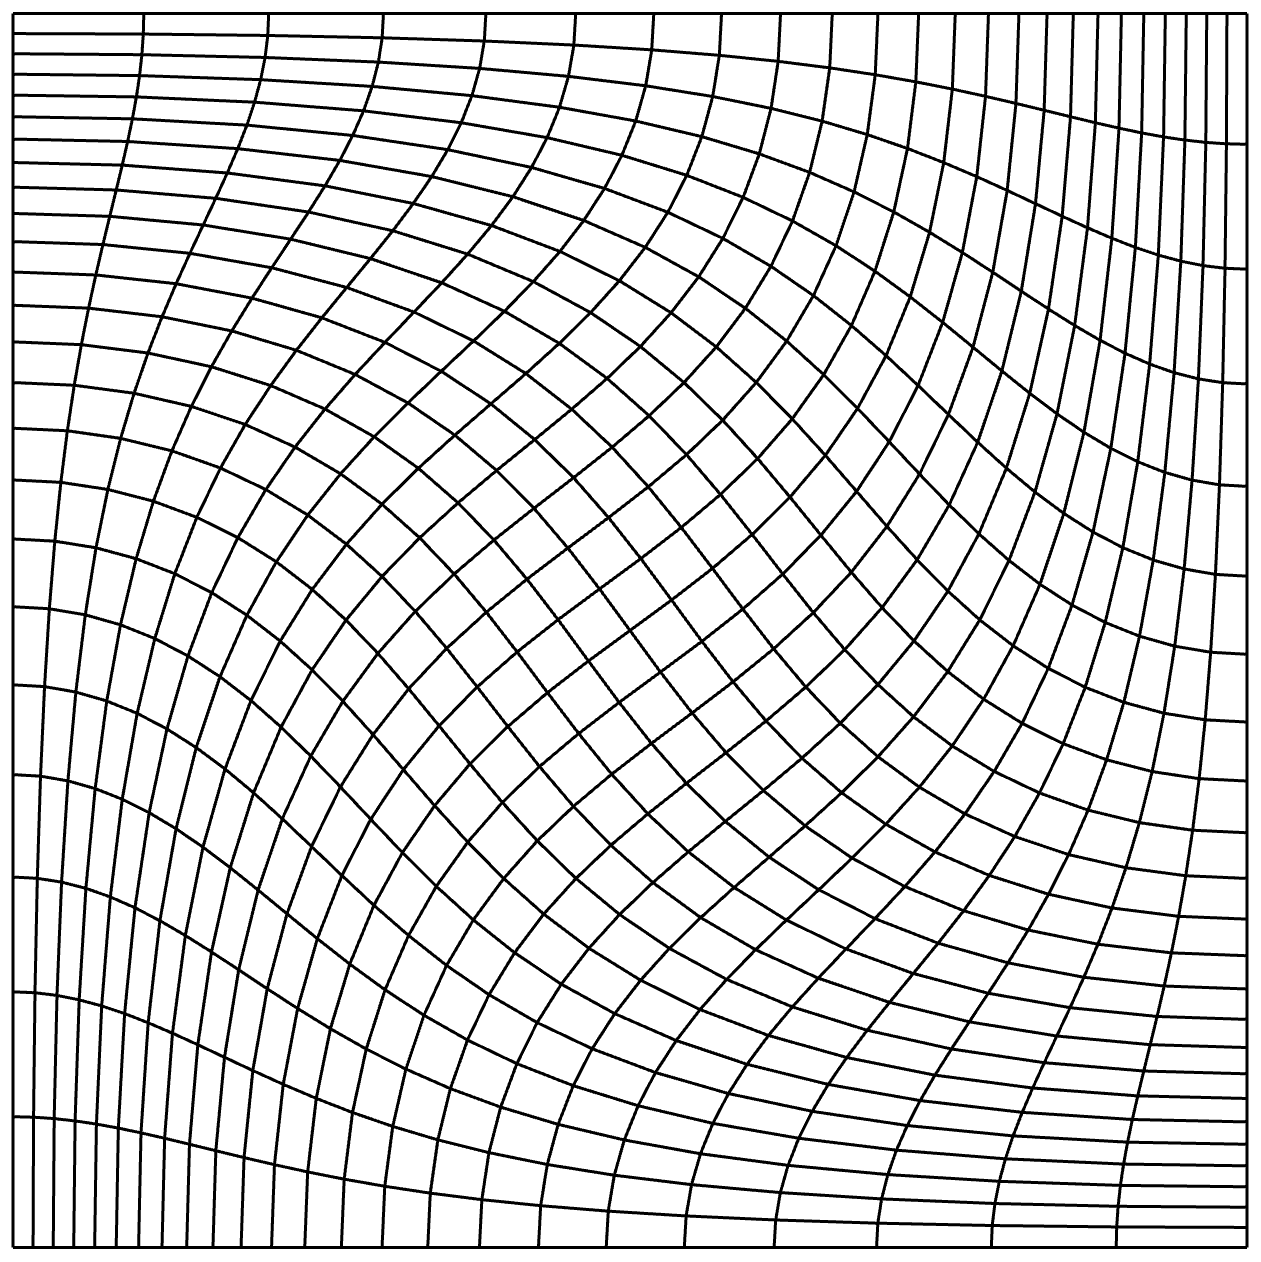
\includegraphics[width=.35\textwidth]{data/img/tgmesh0.3.png}
\caption{A depiction of a third-order mesh generated by distorting an orthogonal mesh according to the Taylor Green vortex. Refinements of this mesh are used in calculating the error with the method of manufactured solutions.}
\label{rtvef:tgmesh}
\end{figure}
We use refinements of a third-order mesh created by distorting an orthogonal mesh according to the velocity field of the Taylor Green vortex. This mesh distortion is generated by advecting the mesh control points with 
	\begin{equation}
		\x = \int_0^T \mat{v} \ud t \,,
	\end{equation}
where the final time $T=0.3\pi$ and 
	\begin{equation}
		\mat{v} = \begin{bmatrix} 
			\sin(x) \cos(y) \\ 
			-\cos(x) \sin(y) 
		\end{bmatrix}
	\end{equation}
is the analytic solution of the Taylor Green vortex. 300 forward Euler steps were used to advect the mesh. An example mesh is shown in Fig.~\ref{rtvef:tgmesh}. Logarithmic regression is used to fit the constant and order of accuracy according to 
	\begin{equation}
		E = C h^{\tilde{p}}
	\end{equation}
where $E$ is the error, $C$ the constant, and $\tilde{p}$ the order of accuracy. Four values of $h$ were used for each MMS problem considered in this section. 
The raw error values are provided in Appendix \ref{chap:mms_data}. 

% --- MMS diffusion --- 
\begin{table}
\centering
\caption{Estimates of the order of accuracy and constant from an isotropic MMS test problem. The H1, RT, and HRT columns refer to the $Y_p\times W_{p+1}$, $Y_p\times \RT_p$, and hybridized $Y_p\times \RT_p$ discretizations, respectively. The error in the scalar flux, the error in the scalar flux when the exact solution is first projected onto $Y_p$, and the error in the current are presented for each method over a range of values of $p$. Here, the VEF data are constant in space and thus are represented exactly. }
\label{rtvef:mms_diff}
\input{figs/rtvef/mms_diff}
\end{table}
We first show the accuracy of the three methods on a simple radiation diffusion problem. The above process is used with $\mat{\Theta} = 0$ so that the angular flux is linearly anisotropic. This forces the Eddington tensor and boundary factor to $\E = \frac{1}{3}\I$ and $E_b = \frac{1}{2}$, mimicking a radiation diffusion problem. Table \ref{rtvef:mms_diff} shows the estimated order of accuracy and constant for $p\in[0,3]$. The error in the scalar flux is computed with two methods: 1) by comparing to the analytic MMS scalar flux solution directly and 2) by projecting the analytic MMS solution onto the corresponding $Y_p$ space. For all orders, the first error measure for the scalar flux converges $\mathcal{O}(h^{p+1})$ while the second converges $\mathcal{O}(h^{p+2})$. This is a mixed finite element superconvergence result that indicates that the nodal values of the scalar flux solution converge one order higher than the $Y_p$ interpolation allows. The current converges as $\mathcal{O}(h^{p+1})$ for all three methods and all orders except for $Y_0 \times W_1$ which converges as $\mathcal{O}(h^{3/2})$ instead of $\mathcal{O}(h)$. On this diffusive problem, the scalar flux and current solutions from the unhybridized and hybridized RT methods are equivalent to machine precision. 

% --- MMS VEF --- 
\begin{table}
\centering
\caption{Estimates of the order of accuracy and constant from a quadratically anisotropic MMS test problem. The H1, RT, and HRT columns refer to the $Y_p\times W_{p+1}$, $Y_p\times \RT_p$, and hybridized $Y_p\times \RT_p$ discretizations, respectively. The error in the scalar flux, the error in the scalar flux when the exact solution is first projected onto $Y_p$, and the error in the current are presented for each method over a range of values of $p$. Here, the angular flux used to calculate the VEF data is represented with $Y_p$. Due to this, the maximum accuracy expected is order $p+1$. }
\label{rtvef:mms_same}
\input{figs/rtvef/mms}
\end{table}
This test is repeated for the quadratically-anisotropic MMS problem (i.e.~using $\mat{\Theta}(\x)$ as defined in Eq.~\ref{rtvef:mmsH}) in Table \ref{rtvef:mms_same}. Since the MMS solution is projected onto $Y_p$, it is expected that this problem can converge at a maximum of order $p+1$. This can be seen in the loss of the superconvergence property. Here, both error measures for the scalar flux converge with $\mathcal{O}(h^{p+1})$. On this transport MMS problem, the current convergence is also reduced. 
Compared to the diffusion case, the H1 current error is maintained for $p$ odd but is reduced by $1/2$ for $p$ even. The RT and HRT methods lose one order for $p$ odd but only half an order for $p$ even. In addition, the RT and HRT discretizations are no longer equivalent to machine precision. This loss of equivalence may be due to inexact numerical quadrature in terms involving the VEF data. The VEF data are improper rational polynomials in space and thus cannot be exactly integrated with Gaussian quadrature. 

% --- MMS elevated psi --- 
\begin{table}
\centering
\caption{Estimates of the order of accuracy and constant from a quadratically anisotropic MMS test problem. The H1, RT, and HRT columns refer to the $Y_p\times W_{p+1}$, $Y_p\times \RT_p$, and hybridized $Y_p\times \RT_p$ discretizations, respectively. The error in the scalar flux, the error in the scalar flux when the exact solution is first projected onto $Y_p$, and the error in the current are presented for each method over a range of values of $p$. Here, the angular flux used to calculate the VEF data is represented with $Y_{p+1}$. Due to this, the maximum accuracy expected is order $p+2$.}
\label{rtvef:mms_elev}
\input{figs/rtvef/mms_elev}
\end{table}
Finally, we repeat the transport MMS problem in the case where the angular flux solution is projected onto $Y_{p+1}$ instead of $Y_p$. This allows a maximum accuracy in the problem of $\mathcal{O}(h^{p+2})$. The estimated orders of convergence and constants are provided in Table \ref{rtvef:mms_elev}. Convergence rates similar to the diffusion problem are observed: the scalar flux solutions converge optimally for all methods and superconvergence of the scalar flux returns. The H1 and HRT methods produce currents that converge at similar rates as in the diffusion case. However, the unhybridized RT method converges suboptimally by one order for $p$ even. The difference in convergence rates between the RT and HRT methods indicates the HRT method is in fact a new discretization for the VEF equations and not simply an algebraic method to reduce the number of globally coupled unknowns. 

\subsection{Thick Diffusion Limit}
The convergence of the VEF methods are investigated in the thick diffusion limit. The material data are set to 
	\begin{equation}
		\sigma_t = 1/\epsilon \,, \quad \sigma_a = \epsilon \,, \quad \sigma_s = 1/\epsilon - \epsilon \,, \quad q = \epsilon \,, 
	\end{equation}
where $\epsilon \in (0,1]$ and the thick diffusion limit corresponds to $\epsilon \rightarrow 0$. We use two coarse meshes that do not resolve the mean free path to stress the convergence of the VEF method. The first is an orthogonal $8\times 8$ mesh with $\D = [0,1]^2$. The second is the triple point mesh shown in Fig.~\ref{rtvef:triple_point_mesh}, a third-order mesh generated with a Lagrangian hydrodynamics code where $\D = [0,7]\times [0,3]$. On the triple point mesh, the angular flux is only approximately inverted due to the lagging of reentrant faces and thus it is expected that convergence will degrade. In addition, highly distorted elements have poor approximation properties. We use Level Symmetric $S_4$ angular quadrature. The three methods are compared when $p=2$. The coupled transport-VEF system is solved with fixed-point iteration. 
% --- triple point mesh --- 
\begin{figure}
\centering
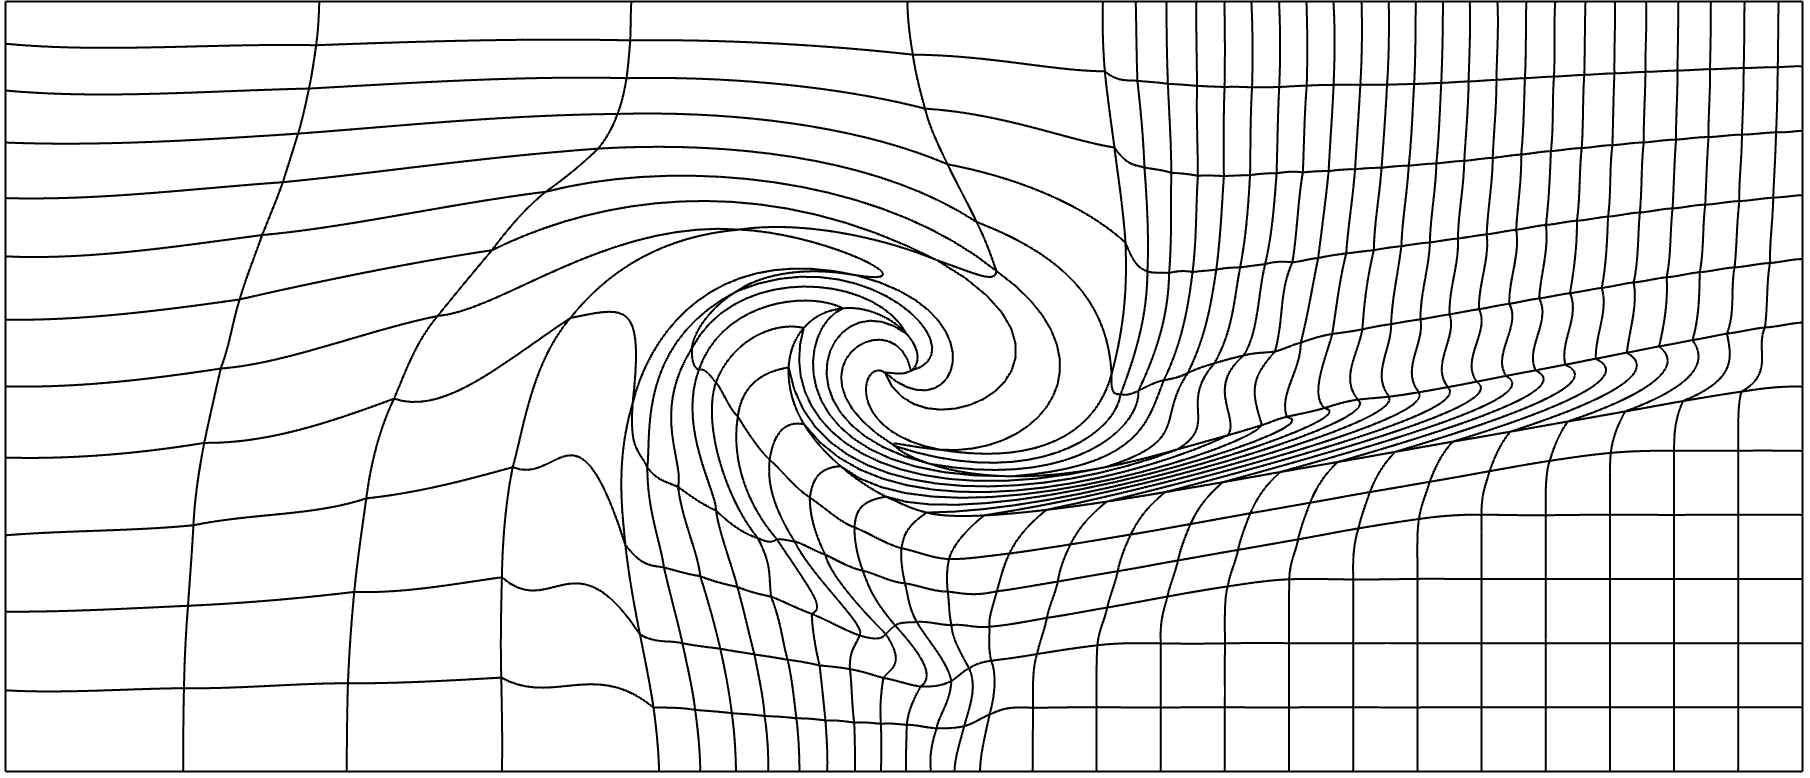
\includegraphics[width=.65\textwidth]{data/img/3point.png}
\caption{A depiction of the triple point mesh used to stress the VEF algorithms on a severely distorted, third-order mesh. This mesh was generated with a Lagrangian hydrodynamics simulation. }
\label{rtvef:triple_point_mesh}
\end{figure}

Table \ref{rtvef:tdl} shows the number of fixed-point iterations until convergence to a tolerance of $10^{-6}$ for each method on the orthogonal and triple point meshes. Rapid convergence is seen for all methods on both problems. The three methods converge equivalently on the orthogonal mesh. On the triple point mesh, the RT and HRT methods converged equivalently. Lineouts of the 2D VEF scalar flux solutions for each method as $\epsilon \rightarrow 0$ are provided in Fig.~\ref{rtvef:eps_lineout} for the orthogonal mesh. In all cases, a non-trivial solution is found. 

% --- thick diffusion limit orthogonal and 3point --- 
\begin{table}
\centering
\caption{The number of fixed-point iterations required for convergence as the thick diffusion limit parameter $\epsilon \rightarrow 0$. The H1, RT, and HRT columns refer to the $Y_2\times W_{3}$, $Y_2\times \RT_2$, and hybridized $Y_2\times \RT_2$ discretizations, respectively. Convergence is tested on an orthogonal $8\times 8$ mesh and on the triple point mesh, a mesh with re-entrant faces. Due to the re-entrant faces, a partial transport sweep is used making convergence slower on the triple point mesh.}
\label{rtvef:tdl}
\input{figs/eps_table_rtvef}
\end{table}

% --- orthogonal lineouts --- 
\begin{figure}
\centering
\foreach \f in {figs/eps_lineout_h1.pdf,figs/eps_lineout_rt.pdf,figs/eps_lineout_hrt.pdf}{
	\begin{subfigure}{.4\textwidth}
	\centering
	\includegraphics[width=\textwidth]{\f}
	\caption{}
	\end{subfigure}	
}
\caption{Lineouts of the 2D solution as $\epsilon\rightarrow 0$. The methods all converge to the asymptotic solution indicating they preserve the thick diffusion limit.}
\label{rtvef:eps_lineout}
\end{figure}

\subsection{Solver Performance on Curved Meshes}
Here, we investigate the robustness of the preconditioned iterative solvers on increasingly distorted meshes. The meshes were created by moving the interior control points of an initially orthogonal, third-order mesh according to the sine distortion: 
	\begin{equation}
		\x = \x + \alpha\begin{bmatrix} 
			\sin(2\pi x) \sin(2\pi y)\\
			\sin(2\pi x) \sin(2\pi y)
		\end{bmatrix} \,,
	\end{equation}
where $\alpha$ controls the amount of distortion. When $\alpha=0$, the mesh is unchanged. The initial mesh was $16\times 16$ with $\D = [0,1]^2$. A range of meshes are shown in Fig.~\ref{rtvef:sine_meshes}. Solver performance is evaluated on the first iteration of the thick diffusion limit problem introduced in the previous section. We use $\epsilon = 10^{-1}$. The number of BiCGStab iterations until convergence to a tolerance of $10^{-6}$ are shown for a range of mesh distortions in Table \ref{rtvef:curved_solvers} for the H1, RT, and HRT VEF methods. The solvers for the RT method did not converge in 250 iterations once the mesh became too distorted. The H1 discretization converged on all the meshes tested but the iteration counts varied between 46 and 69 whereas HRT was solved more uniformly, varying only between 7 and 11 iterations. This indicates the solvers for the RT method are sensitive to mesh distortion. 
% --- sine distortions --- 
\begin{figure}
\centering
\begin{subfigure}{.24\textwidth}
	\centering
	
\includegraphics[width=\textwidth]{data/img/sine0.png}
	\caption{$\alpha = 0.000$}
\end{subfigure}\enspace
\begin{subfigure}{.24\textwidth}
	\centering
	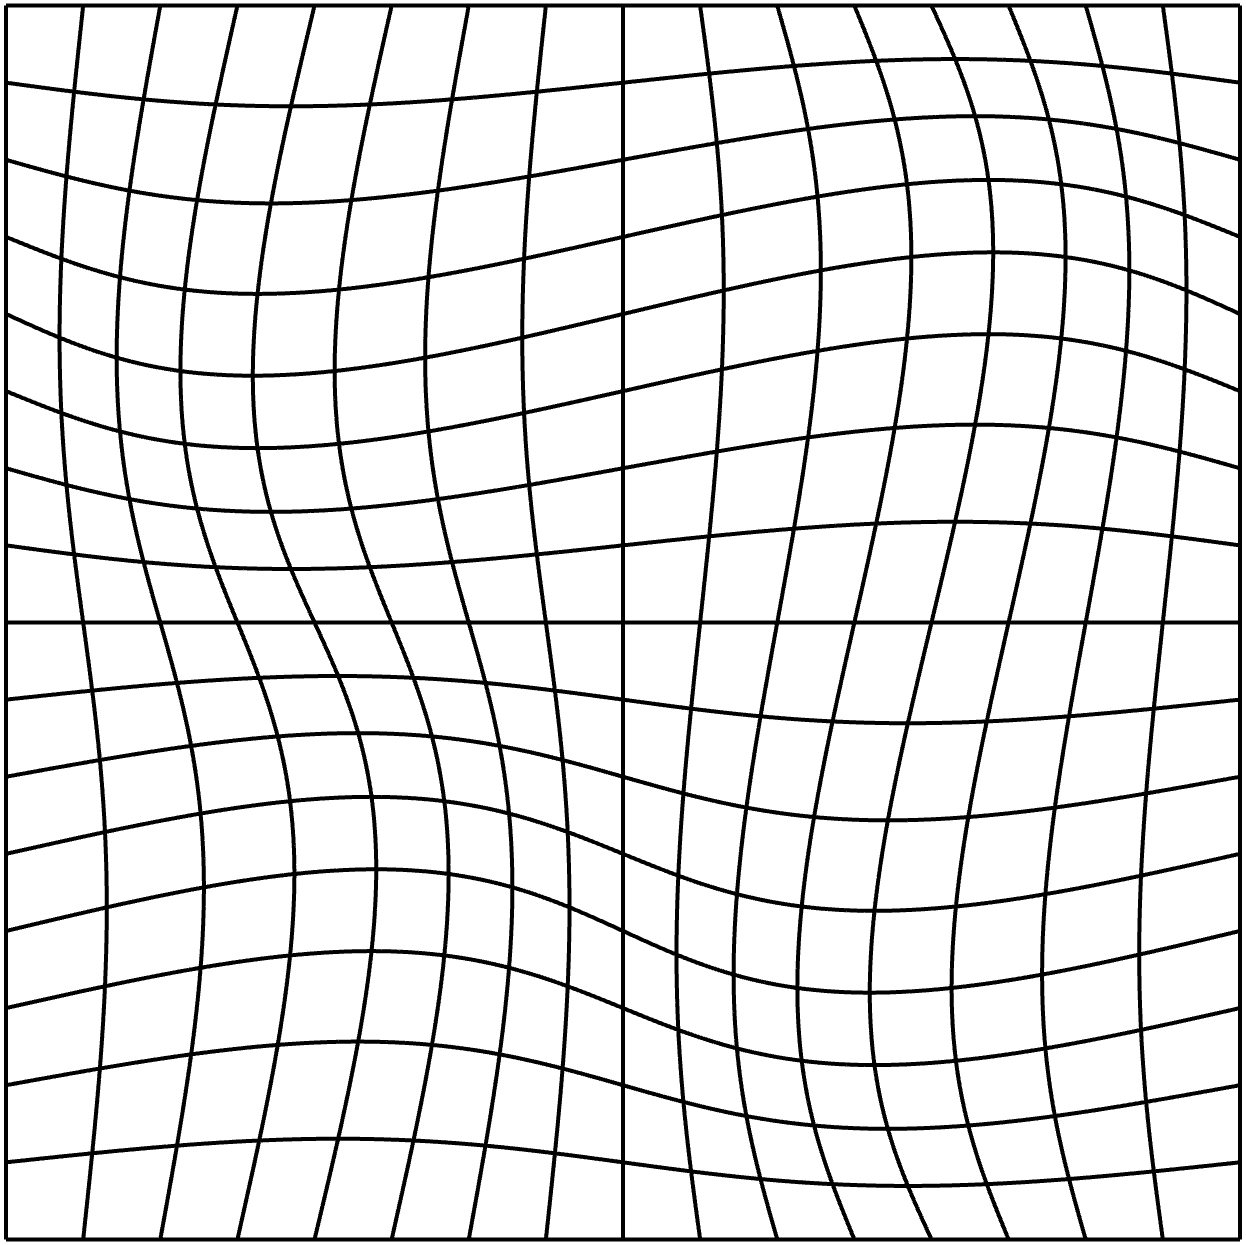
\includegraphics[width=\textwidth]{data/img/sine50.png}
	\caption{$\alpha = 0.050$}
\end{subfigure}\enspace
\begin{subfigure}{.24\textwidth}
	\centering
	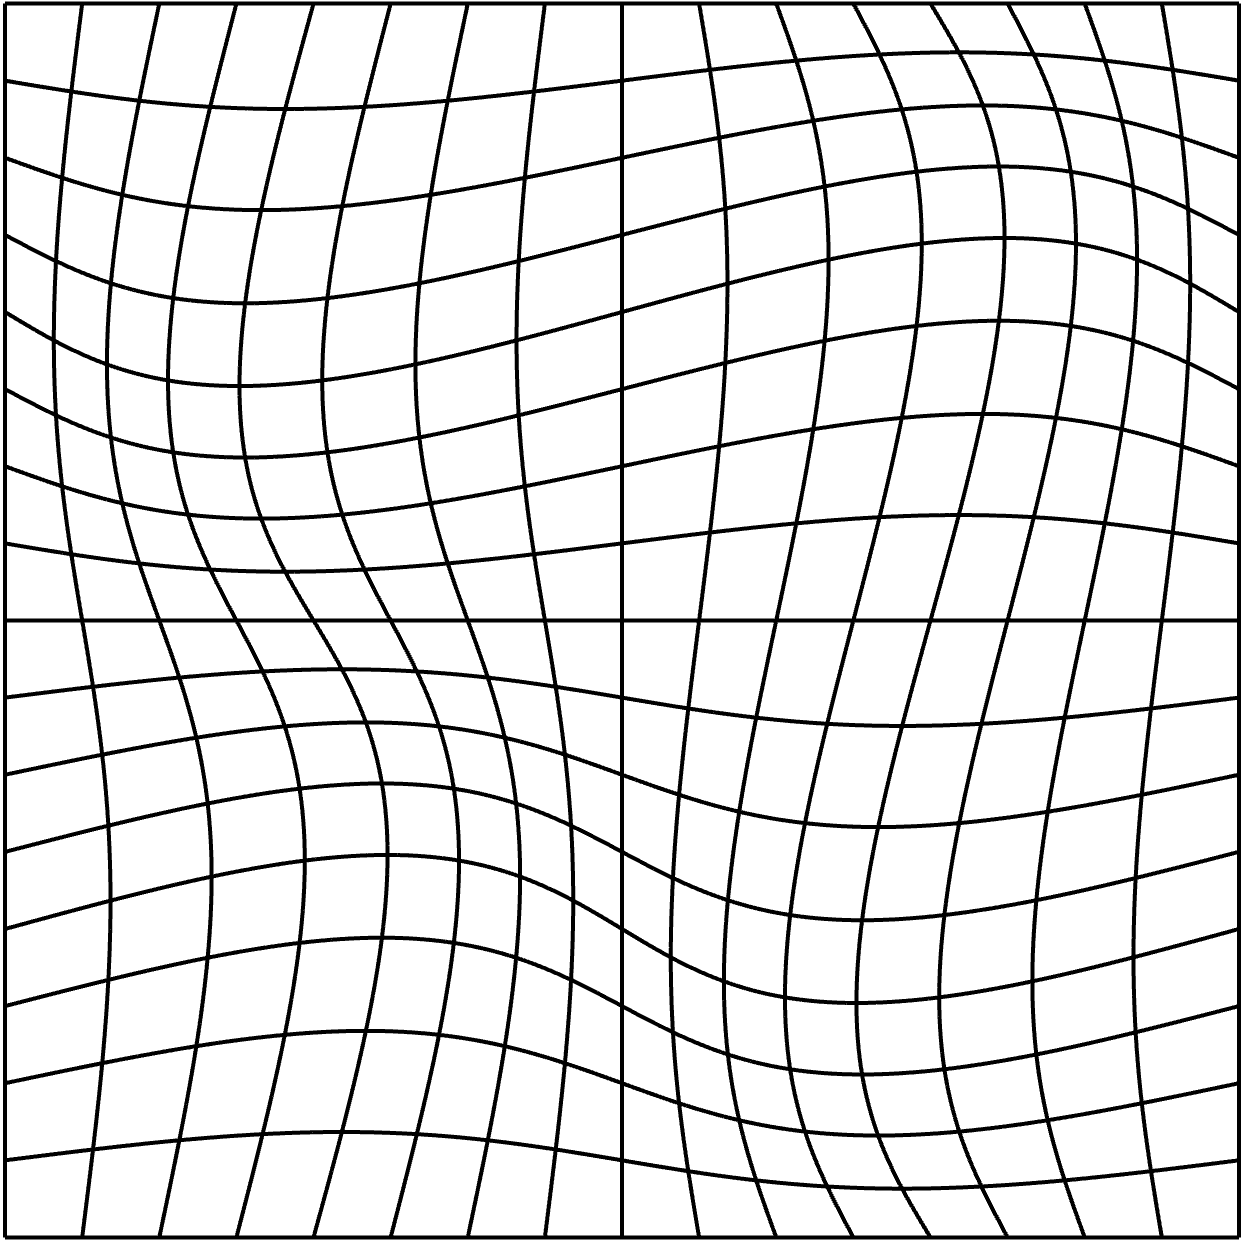
\includegraphics[width=\textwidth]{data/img/sine60.png}
	\caption{$\alpha = 0.060$}
\end{subfigure}\enspace
\begin{subfigure}{.24\textwidth}
	\centering
	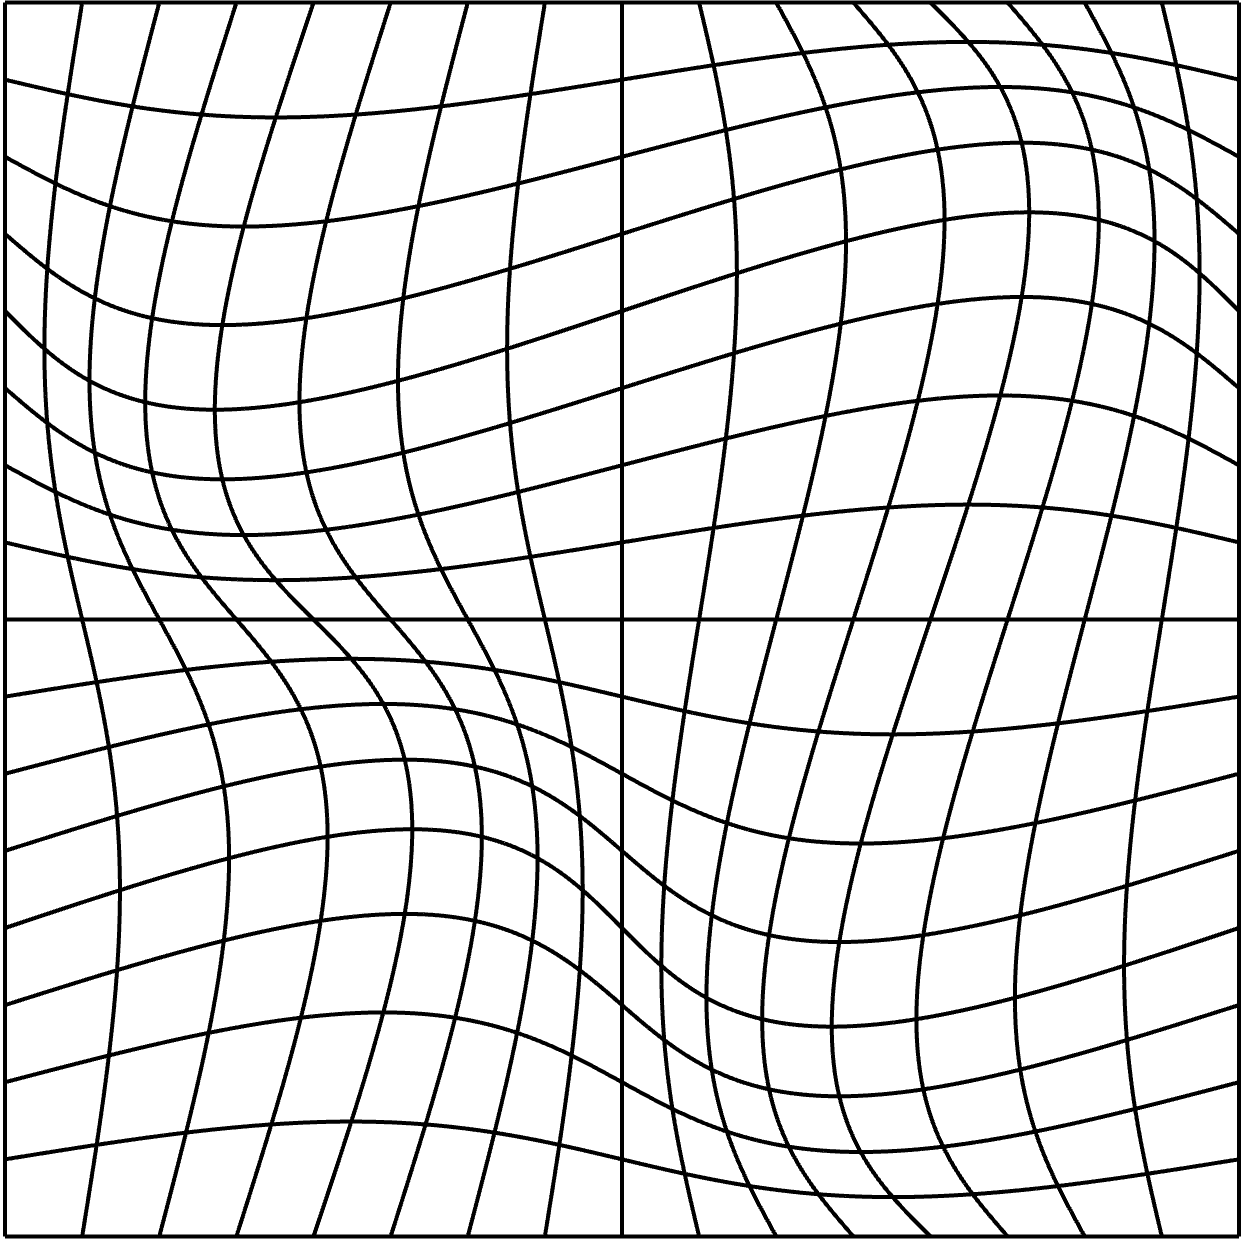
\includegraphics[width=\textwidth]{data/img/sine80.png}
	\caption{$\alpha = 0.080$}
\end{subfigure}
\caption{A selection of meshes generated by distorting a third-order, orthogonal $16\times 16$ mesh according to the sine distortion. The parameter $\alpha$ controls the amount of distortion. These meshes are used to assess linear solver robustness against mesh distortion. }
\label{rtvef:sine_meshes}
\end{figure}

% --- curved solvers --- 
\begin{table}
\centering
\caption{Number of BiCGStab iterations until convergence on the first iteration of a thick diffusion limit problem with $\epsilon = 10^{-1}$ as the mesh distortion parameter increases. A $--$ indicates BiCGStab did not converge in 250 iterations. Here, H1, RT, and HRT rows refer to the $Y_p\times W_{p+1}$, $Y_p\times \RT_p$, and hybridized $Y_p\times \RT_p$ discretizations, respectively.}
\label{rtvef:curved_solvers}
\input{figs/rtvef/solvers}
\end{table}

\subsection{Crooked Pipe} \label{rtvef_sec:cp}
We now show convergence in outer fixed-point iterations and inner preconditioned linear solver iterations on a more realistic, multi-material problem. The geometry and materials are shown in Fig.~\ref{rtvef:cp_diag}. The problem consists of two materials, the wall and the pipe, which have an 1000x difference in total interaction cross section. Time dependence is mocked by including artificial absorption and sources that correspond to backward Euler time integration. The time step is set so that $c\Delta t = 10^3$ and the initial condition is $\psi_0 = 10^{-4}$. The absorption and source are then $\sigma_a = 1/c\Delta t = 10^{-3} \si{\per\cm}$ and $q = \psi_0/c\Delta t = 10^{-1} \si{\per\cm\cubed\per\s\per\str}$. The boundary conditions are set so that isotropic inflow of magnitude $1/2\pi$ enters on the left entrance of the pipe. A Level Symmetric S$_{12}$ angular quadrature set is used. The quadratic programming negative flux fixup from \cite{YEE2020109696} is used inside the transport sweep to ensure positivity so that the VEF data are well defined. 
% --- crooked pipe geometry --- 
\begin{figure}
\centering
\includegraphics[width=.65\textwidth]{figs/crooked_pipe.pdf}
\caption{The geometry, material data, and boundary conditions for the linearized crooked pipe problem. }
\label{rtvef:cp_diag}
\end{figure}

The outer fixed-point and inner linear iterative efficiency are shown by refining in $h$ and $p$ on an orthogonal mesh. Anderson acceleration with two Anderson vectors is used. The previous outer iteration's solution is used as an initial guess for the inner solver so that the initial guess becomes progressively more accurate as the outer iteration converges. The outer tolerance is $10^{-6}$ and the inner BiCGStab tolerance is $10^{-8}$. 

Table \ref{rtvef:cp} shows the number of Anderson-accelerated fixed-point iterations to convergence and the maximum, minimum, and average number of inner iterations performed across all outer iterations for the H1, RT, and HRT methods. The RT and HRT methods had equivalent convergence in outer iterations with H1 requiring up to 15 more iterations. The slowdown of H1 is likely caused by its increased reliance on the negative flux fixup compared to the RT and HRT methods. The RT and HRT inner solvers were scalable in $h$ and $p$ while the H1 solvers were not. On the problem with the smallest value of $h$, the H1 inner solver did not converge within 100 iterations on at least one of the solves. 
% --- crooked pipe hp scaling --- 
\begin{table}
\centering
\caption{The number of outer Anderson-accelerated fixed-point iterations until convergence along with the maximum, minimum, and average numbers of inner BiCGStab iterations until convergence on the linearized crooked pipe problem. Two Anderson vectors were used. The H1, RT, and HRT columns refer to the $Y_p\times W_{p+1}$, $Y_p\times \RT_p$, and hybridized $Y_p\times \RT_p$ discretizations, respectively. The H1 and RT methods were preconditioned with a block lower triangular preconditioner with AMG applied to the lumped Schur complement. HRT was preconditioned with AMG. The previous outer iteration's solution was used as the initial guess for the inner iteration. }
\label{rtvef:cp}
\begin{adjustbox}{max width=\textwidth}
\input{figs/cp.tex}
\end{adjustbox}
\end{table}

\subsection{Eigenvalue Problem} \label{rtvef_sec:badmodes}
It was observed that the $Y_p \times W_{p+1}$ discretization exhibited poor solution quality in under resolved problems and could not be scalably solved using block preconditioners. In particular, AMG struggled to adequately precondition the lumped Schur complement. To investigate this issue, we consider the following eigenvalue problem: 
	\begin{equation}
		-\nabla^2 u = \lambda u \,, \quad \x \in \D\,, 
	\end{equation}
	\begin{equation}
		u = 0 \,, \quad \x \in \partial \D \,,
	\end{equation}
with $\D = [0,1]^2$. 
The exact solutions are 
	\begin{equation}
		u = \sin(k_x \pi x) \sin(k_y \pi y) \,, \quad \lambda = \pi^2(k_x^2 + k_y^2) \,. 
	\end{equation}
The $Y_1 \times W_2$ discretization's lumped Schur complement is used to discretize this problem as: find $u \in Y_1$ such that 
	\begin{equation}
		\tmat{S} \fevec{u} = \lambda \mat{M} \fevec{u} \,,
	\end{equation}
where $\mat{M}$ is the $Y_1$ mass matrix. The Locally Optimal Block Preconditioned Conjugate Gradient (LOBPCG) solver from \emph{hypre} was used to solve for the first 5 eigenvalues and eigenvectors of this system. The solver correctly found the first four eigenvalues and eigenvectors but produced the high-frequency, ``checkerboard'' mode shown in Fig.~\ref{rtvef:badmode} for the fifth. This checkerboard mode corresponded to a non-physically degenerate eigenvalue of $8\pi^2$. The presence of this mode indicates the $Y_p \times W_{p+1}$ discretization allows non-physical, spurious modes that are slowly decaying and high frequency. Such modes are slow to remove with relaxation and also cannot be accurately represented on a coarser grid, meaning AMG will not be an effective preconditioner. 
% --- bad mode plot --- 
\begin{figure}
\centering
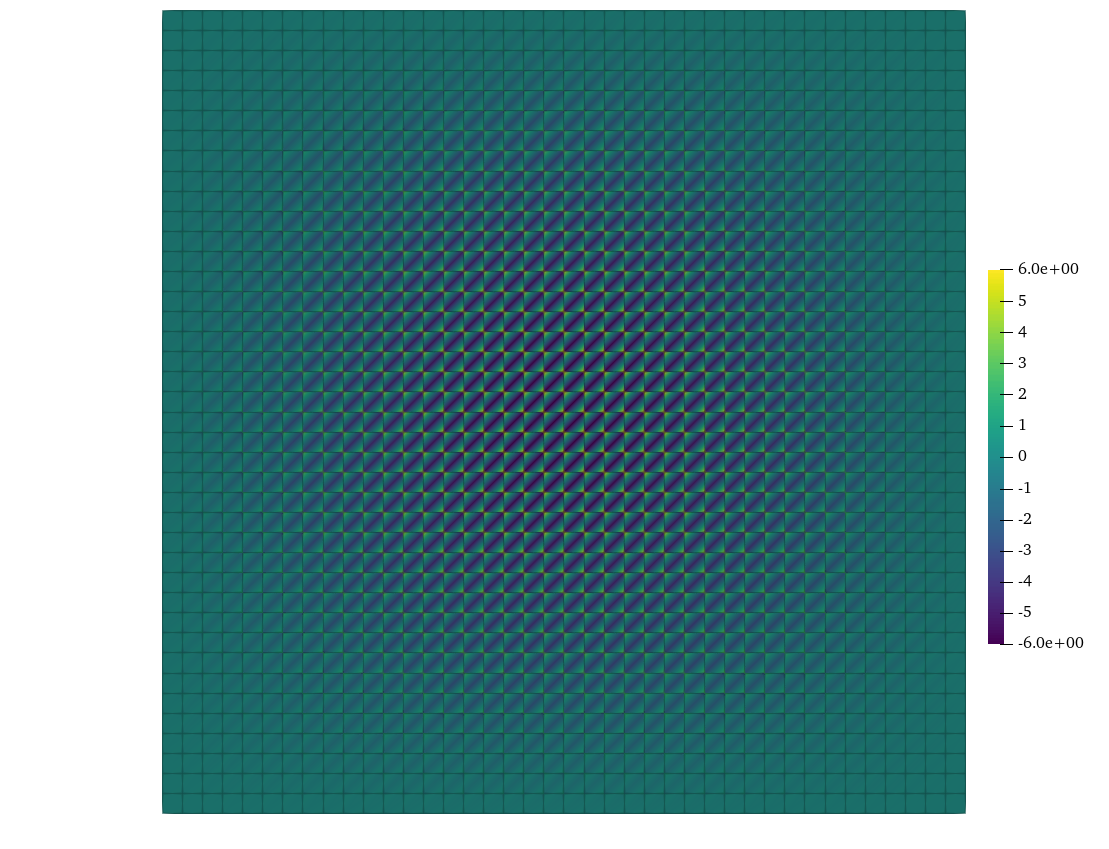
\includegraphics[width=.5\textwidth]{data/img/badmode40.png}
\caption{A depiction of an eigenmode corresponding to an eigenvalue of $8\pi^2$ of the Poisson eigenvalue problem discretized with the $Y_1\times W_2$ discretization's lumped Schur complement. For this eigenvalue, the exact solution is $\sin(2\pi x)\sin(2\pi y)$ meaning this mode is spurious. The presence of high-frequency spurious modes in the $Y_p\times W_{p+1}$ discretization's lumped Schur complement degrades the effectiveness of AMG and thus the performance of the block preconditioners used to solve the full $Y_p\times W_{p+1}$ discretization.}
\label{rtvef:badmode}
\end{figure}

\subsection{Weak Scaling} \label{rtvef_sec:weak}
Finally, we show that the RT and HRT methods scale in parallel. The parallel partitioning is such that there are $\approx\!\num{9000}$ VEF scalar flux unknowns per processor. The results were generated on 32 nodes of the \texttt{rztopaz} machine at LLNL which has two 18-core Intel Xeon E5-2695 CPUs per node. The materials and geometry from the crooked pipe in Section \ref{rtvef_sec:cp} are used. In Table \ref{rtvef:weak}, the number of BiCGStab iterations until convergence to a tolerance of $10^{-8}$ is shown when 1) a transport solve is used to compute the VEF data and 2) the VEF data are set to their thick diffusion limit values of $\E = \frac{1}{3}\I$ and $E_b = \frac{1}{2}$. The RT and HRT discretizations were used with $p=2$. Both the RT and HRT methods are scalable in parallel out to over 10 million scalar flux unknowns. Compared to the corresponding diffusion problems, HRT required at most 5 more iterations to solve the VEF equations while RT required at most 9 more iterations. 
% --- weak scaling --- 
\begin{table}
\centering
\caption{A weak scaling study on the first iteration of the linearized crooked pipe problem. The RT and HRT columns refer to the $Y_2\times \RT_p$ and hybridized $Y_2\times \RT_P$ discretizations, respectively. The RT method uses lower block triangular preconditioning with AMG on the lumped Schur complement. HRT is preconditioned with AMG. BiCGStab iteration counts are compared when a parallel block Jacobi sweep is used to compute the VEF data (VEF) and when the VEF data are set to mock a radiation diffusion problem (Diffusion). The DOF column corresponds to the number of VEF scalar flux unknowns.}
\label{rtvef:weak}
\input{figs/rtvef/weak}
\end{table}

\end{document}